%%%%%%%%%%%%%%%%%%%%%%%%%%%%%%%%%%%%%%%%%%%%%%%
%
% Template per Elaborato di Laurea
% DISI - Dipartimento di Ingegneria e Scienza dell’Informazione
%
%
% Per la generazione corretta del 
% pdflatex nome_file.tex
%
%%%%%%%%%%%%%%%%%%%%%%%%%%%%%%%%%%%%%%%%%%%%%%%

% formato FRONTE RETRO
\documentclass[epsfig,a4paper,11pt,titlepage,twoside,openany]{book}
\usepackage{epsfig}
\usepackage{plain}
\usepackage{setspace}
\usepackage{caption}
\usepackage{subcaption}
\usepackage{url}
\usepackage[breaklinks]{hyperref}
\def\UrlBreaks{\do\/\do-}
\usepackage{amsmath}
\usepackage{graphicx}
\usepackage[export]{adjustbox}

\DeclareCaptionFormat{citation}{%
  \ifx\captioncitation\relax\relax\else
    \captioncitation\par
  \fi
  #1#2#3\par}
\newcommand*\setcaptioncitation[1]{\def\captioncitation{\textit{Source:}~#1}}
\let\captioncitation\relax
\captionsetup{format=citation,justification=centering}
\usepackage[paperheight=29.7cm,paperwidth=21cm,outer=1.5cm,inner=2.5cm,top=2cm,bottom=2cm]{geometry} % per definizione layout
\usepackage{titlesec} % per formato custom dei titoli dei capitoli

%%%%%%%%%%%%%%
% supporto lettere accentate
%
%\usepackage[latin1]{inputenc} % per Windows;
\usepackage[utf8x]{inputenc} % per Linux (richiede il pacchetto unicode);
%\usepackage[applemac]{inputenc} % per Mac.

\singlespacing

\usepackage[english]{babel}

\begin{document}

  % nessuna numerazione
  \pagenumbering{gobble} 
  \pagestyle{plain}

\thispagestyle{empty}

\begin{center}
  \begin{figure}[h!]
    \centerline{
\psfig{file=marchio_unitrento_colore_it_202002.eps,width=0.6\textwidth}}
  \end{figure}

  \vspace{2 cm} 

  \LARGE{Department of Information Engineering and Computer Science\\}

  \vspace{1 cm} 
  \Large{Computer, Communications and Electronic Engineering Degree\\
  }

  \vspace{2 cm} 
  \Large\textsc{Final paper\\} 
  \vspace{1 cm} 
  \Huge\textsc{Continual Learning on Max78000\\}
  \Large{\it{Application of Online Learning technique}}


  \vspace{2 cm} 
  \begin{tabular*}{\textwidth}{ c @{\extracolsep{\fill}} c }
  \Large{Supervisors} & \Large{Student}\\
  \Large{Prof. Kasim Sinan Yildirim}& \Large{Giovanni Lunardi}\\
  \Large{Prof. Davide Brunelli}& \\
  \Large{Khakim Akhunov}& \\
  \Large{Luca Caronti}
  \end{tabular*}

  \vspace{2 cm} 

  \Large{Academic year 2021/2022}
  
\end{center}



  \clearpage
 
%%%%%%%%%%%%%%%%%%%%%%%%%%%%%%%%%%%%%%%%%%%%%%%%%%%%%%%%%%%%%%%%%%%%%%%%%%
%%%%%%%%%%%%%%%%%%%%%%%%%%%%%%%%%%%%%%%%%%%%%%%%%%%%%%%%%%%%%%%%%%%%%%%%%%
%% Nota
%%%%%%%%%%%%%%%%%%%%%%%%%%%%%%%%%%%%%%%%%%%%%%%%%%%%%%%%%%%%%%%%%%%%%%%%%%
%% Sezione Ringraziamenti opzionale
%%%%%%%%%%%%%%%%%%%%%%%%%%%%%%%%%%%%%%%%%%%%%%%%%%%%%%%%%%%%%%%%%%%%%%%%%%
%%%%%%%%%%%%%%%%%%%%%%%%%%%%%%%%%%%%%%%%%%%%%%%%%%%%%%%%%%%%%%%%%%%%%%%%%%
  \thispagestyle{empty}

\begin{center}
  {\bf \Huge Acknowledgements}
\end{center}

\vspace{4cm}

\emph{
  Before proceeding with the discussion, I would like to dedicate a few lines to all those who have been close to me in this journey of personal and professional growth. I feel obliged to dedicate this page of this paper to the people who supported me in writing it. 
 }\\
 \emph{
  First of all, I heartfelt thank you to my supervisors Yildirim Kasim Sinan, Brunelli Davide, Luca Caronti, and Khakim Akhunov who were always ready to give me the right guidance at every stage of the realization of the paper. Thanks to you, I have increased my knowledge and skills.
} \\
  \emph{
  I thank my family, especially my parents, because without them I could never have embarked on this course of study. They have always supported me throughout my university journey.
  }\\
  \emph{
  I thank my girlfriend Sara for passing on her immense strength and courage to me. Thank you for all the time you have given me. Thank you for always being there.
  }\\
  \emph{
  Finally, I would like to dedicate this achievement to myself for never giving up even in the most difficult times. May it be the beginning of a long and brilliant professional career.
}

  \clearpage
  \pagestyle{plain} % nessuna intestazione e pie pagina con numero al centro

  
  % inizio numerazione pagine in numeri arabi
  \mainmatter

%%%%%%%%%%%%%%%%%%%%%%%%%%%%%%%%%%%%%%%%%%%%%%%%%%%%%%%%%%%%%%%%%%%%%%%%%%
%%%%%%%%%%%%%%%%%%%%%%%%%%%%%%%%%%%%%%%%%%%%%%%%%%%%%%%%%%%%%%%%%%%%%%%%%%
%% Nota
%%%%%%%%%%%%%%%%%%%%%%%%%%%%%%%%%%%%%%%%%%%%%%%%%%%%%%%%%%%%%%%%%%%%%%%%%%
%% Si ricorda che il numero massimo di facciate e' 30.
%% Nel conteggio delle facciate sono incluse 
%%   indice
%%   sommario
%%   capitoli
%% Dal conteggio delle facciate sono escluse
%%   frontespizio
%%   ringraziamenti
%%   allegati    
%%%%%%%%%%%%%%%%%%%%%%%%%%%%%%%%%%%%%%%%%%%%%%%%%%%%%%%%%%%%%%%%%%%%%%%%%%
%%%%%%%%%%%%%%%%%%%%%%%%%%%%%%%%%%%%%%%%%%%%%%%%%%%%%%%%%%%%%%%%%%%%%%%%%%

    % indice
    \tableofcontents
    \clearpage
    
    
          
    % gruppo per definizone di successione capitoli senza interruzione di pagina
    \begingroup
      % nessuna interruzione di pagina tra capitoli
      % ridefinizione dei comandi di clear page
      \renewcommand{\cleardoublepage}{} 
      \renewcommand{\clearpage}{} 
      % redefinizione del formato del titolo del capitolo
      % da formato
      %   Capitolo X
      %   Titolo capitolo
      % a formato
      %   X   Titolo capitolo
      
      \titleformat{\chapter}
        {\normalfont\Huge\bfseries}{\thechapter}{1em}{}
        
      \titlespacing*{\chapter}{0pt}{0.59in}{0.02in}
      \titlespacing*{\section}{0pt}{0.20in}{0.02in}
      \titlespacing*{\subsection}{0pt}{0.10in}{0.02in}
      
      % sommario
      \chapter*{Summary}
\label{Summary}

\quad Recently, many applications have begun to use a branch of Machine Learning called TinyML. This paper exploits a new system based on this technology. Specifically, the application implements a Continual Learning (CL) system on the Max78000 board, a new breed of AI microcontroller built to enable neural networks to execute at ultra-low power and live at the edge of IoT. Via a CL system, the application learns a new class with small and efficient training. The entire network model is a CNN system that runs on a hardware-based accelerator. 

\clearpage
\newpage
\mbox{~}
\clearpage
\newpage




%%%%%%%%%%%%%%%%%%%%%%%%%%%%%%%%%%%%%%%%%%%%%%%%%%%%%%%%%%%%%%%%%%%%%%%%%%
%%%%%%%%%%%%%%%%%%%%%%%%%%%%%%%%%%%%%%%%%%%%%%%%%%%%%%%%%%%%%%%%%%%%%%%%%%
%% Nota
%%%%%%%%%%%%%%%%%%%%%%%%%%%%%%%%%%%%%%%%%%%%%%%%%%%%%%%%%%%%%%%%%%%%%%%%%%
%% Sommario e' un breve riassunto del lavoro svolto dove si descrive 
%% l’obiettivo, l’oggetto della tesi, le metodologie e 
%% le tecniche usate, i dati elaborati e la spiegazione delle conclusioni 
%% alle quali siete arrivati.
%% Il sommario dell’elaborato consiste al massimo di 3 pagine e deve contenere le seguenti informazioni: 
%%   contesto e motivazioni
%%   breve riassunto del problema affrontato
%%   tecniche utilizzate e/o sviluppate
%%   risultati raggiunti, sottolineando il contributo personale del laureando/a
%%%%%%%%%%%%%%%%%%%%%%%%%%%%%%%%%%%%%%%%%%%%%%%%%%%%%%%%%%%%%%%%%%%%%%%%%%
%%%%%%%%%%%%%%%%%%%%%%%%%%%%%%%%%%%%%%%%%%%%%%%%%%%%%%%%%%%%%%%%%%%%%%%%%%      
      
      %%%%%%%%%%%%%%%%%%%%%%%%%%%%%%%%
      % lista dei capitoli
      %
      % \input oppure \include
      %
      \chapter{Introduction}
\label{cha:introduction}

\quad In recent years Machine Learning (ML) applications on small devices, known as TinyML, have been widely used. This kind of technology has been used in almost every sector even in automation, industrial applications, and autonomous driving. Another well-suited field for TinyML is the Internet of Things (IoT). Here edge computing technology is applied to the embedded systems to perform fast and high-level Data computation. This shift comes with great benefits but also some challenges. Firstly, it drastically reduces the traffic on the IoT network. Secondly, the model runs on the edge of the network. (This way it is not necessary to send the Data to a server to run inference [and it reduces the latency of the output]). Not moving Data around allow embedded systems to use less power and concentrate the energy consumption on the inference. Also, microcontrollers have low power consumption. Less internet bandwidth is used to manage the Data hence they do not have to be sent to the server constantly. Data are stored only on the edge, so that in addition, it is safer when talking about privacy.

\quad In the last few decades, (CNN) Convolution Neural Networks have been the customary technology in many image-related machine learning algorithms given their high accuracy in image recognition.
Advancements in Machine Learning, especially Deep Learning, have entirely revolutionized the tech world and society. Tasks that were considered impossible to be performed by machines are now the foundation of many intelligent objects surrounding us. However, the classical machine learning paradigm consists of collecting a massive volume of Data, training the model, and eventually deploying it, a method that is progressively becoming too obsolete to deal with current problems. Thanks to a new branch of ML called Continual Learning, (or Online Learning), we can address the issue of not having all the Data at once during training and the inability to adjust to changing scenarios. This new technique is built on the idea of learning continuously and adaptively about the external world, collecting Data through time. Therefore it allows the model to change and fine-tune its weights and structure to better contrast the change in context. An additional feature is the ability to recognize new never-seen classes. This characteristic, if paired with the model's ability to extend its structure, allows the creation of a flexible model that can allocate brand new weights and biases for better predictions.


\section{Problem Statement}
\label{sec:problem_statement}
\quad The implementation of CL in industrial applications is not a new topic in the research world, but its application on tiny devices has just started to become increasingly popular. The purpose is to adapt a simplified version of the continual learning algorithm to a microcontroller (MCU) equipped with a CNN accelerator. The procedure is applied to a Mnist image recognition model whose weights will change to be able to recognize a new class. The source of samples Data is the Emnist dataset, a collection of handwritten black and white images. The system replaces an existing class with a never-seen one, and continually performs updates on weights and biases for flexible adaptation to the new one. The experiment aims to execute real-time training to let the ML model learn a new pattern. The study can be considered a simplification of real-world applications, but it is a clear example of how a CL model can behave in these scenarios. The work carried out in this study shows that the application on tiny devices is possible. Even though the CL strategies are applied only on the last layer the results are satisfying and in the example, the model correctly digests the new class. The test shows that a model equipped with a CL system can expand its knowledge and learn more classes, in this case, a letter.
The MCU where the algorithm is implemented is the Max78000 board made by Maxim company.  

\section{Brief Summary}
\label{sec:brief_summary}

\quad This thesis is divided into chapters. The first chapter introduces a background of what was the preliminary study for the conduction of this project. The second chapter, on the other hand, discusses the steps in the implementation of the system, starting with the creation of the project template and the study behind the allocation of weights, and ending with the main pipeline of the system and an explanation of the algorithm used. The last chapter talks about the practical aspects of the experiment such as the network model and the device set up, afterwards it also discusses the results obtained and demonstrates some of them with graphs.

\clearpage
\newpage
\mbox{~}
\clearpage
\newpage
      \chapter{Background}
\label{cha:Background}
\quad Machine Learning (ML) is a field of inquiry devoted to understanding and building methods that learn, methods that leverage data to improve performance on certain set of tasks. It deals with the creation and training of models that can learn from data. An ML model is a file produced from a training procedure built with specific characteristics. The base ML model is composed of neurons grouped inside layers, connected in series (as pictured in figure \ref{base_neural_network}). The layers can be divided into the input layer, hidden layer, and output layer. The first layer, which is the input one, has the task of taking an input array (usually a matrix) where each neuron in the layer represents a value of the input. The following steps are hidden layers that take a certain number of input and convolute them with values called weights. Upcoming there are the output layers which depending on the model can represent different types of information such as bounding box or percentages representing classification.   

\begin{figure}[!ht]
\centerline{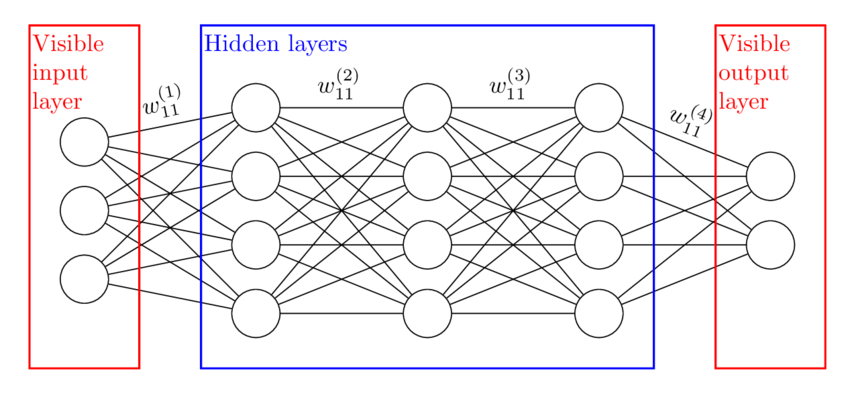
\psfig{file=Images/An-example-of-a-deep-learning-neural-network-with-3-hidden-layers.png,width=0.8\textwidth}}
\caption{Example of layers inside a base ML model \cite{Quantum_machine_learning}}
\label{base_neural_network}
\end{figure}

\section{Convolutional Neural Network}
\label{sec:context}
\quad The network taken into account in this paper is a convolution model, a Supervised Deep Learning model used for Computer Vision. The base operator is the neuron that grasps inputs and throughout operations gives an output. The differences between a NN and a CNN are the convolutional layers used to apply the convolution operation on images and thee pooling layers used to downsize the images through each layer (figure \ref{cnn_neural_network}). These two together encompass feature selection (extraction). Weights are also applied differently than the base model because they are allocated into kernels. Each kernel is used to filter a smaller area of the matrix given by the previous layer. The result is called a feature map. At each iteration, the kernel computes the convolution in a given area and then it slides off by a  value called stride. The last set of layers is the Fully Connected Layers (FC layer) which are a combination of Affine function and Non-linear functions such as Sigmoid, TanH, and ReLu. A Fully Connected Layer takes input from a flattened layer, a one-dimensional layer (1D layer). The data coming from the flattened layer is passed first to the Affine function and then to the non-linear one. In the end, is the softmax function that adds up the values to their corresponding final result and outputs the percentage of each class.

\begin{figure}[!ht]
\centerline{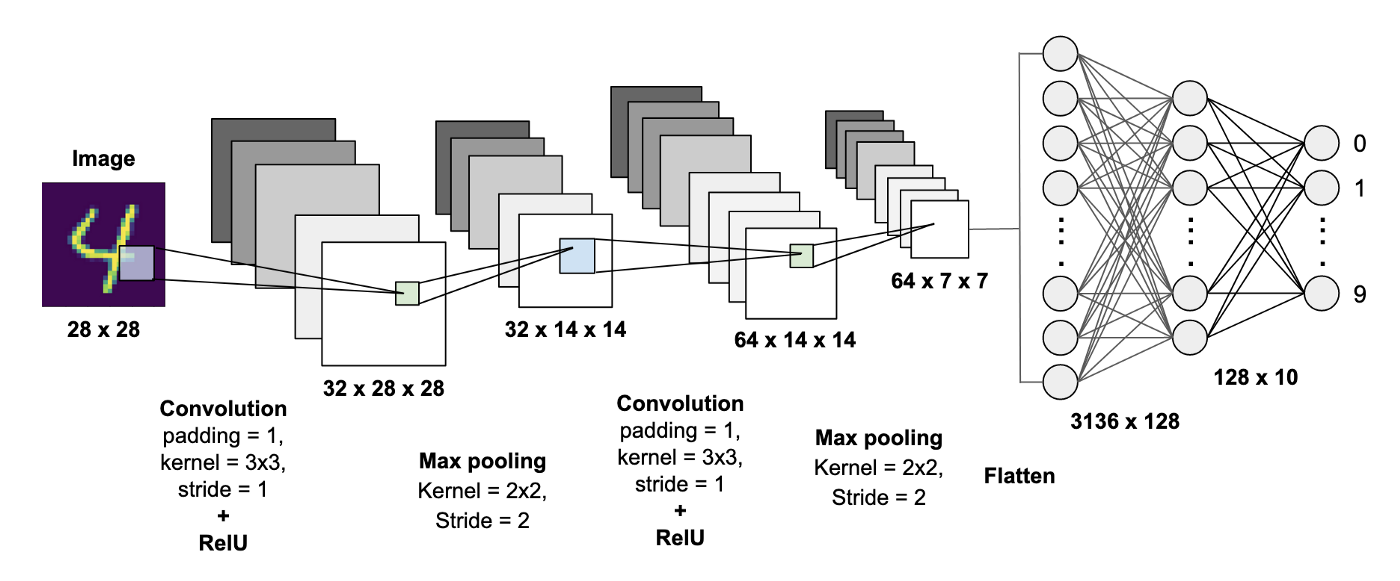
\psfig{file=Images/An-example-of-convolution-neural-network.png,width=0.8\textwidth}}
\setcaptioncitation{https://miro.medium.com/max/1400/1*SGPGG7oeSvVlV5sOSQ2iZw.png}
\caption{Example of layers inside a CNN model}
\label{cnn_neural_network}
\end{figure}

\section{Continual on-line learning}
\label{sec:CL}
\quad Machine learning applications base their functionality on the use of trained models for the elaboration of Data. One of the main aspects of ML applications is their capability to perform only inference over input samples. These systems are implemented with the only purpose of performing inference which is a sufficient requirement for typical applications. However, the usage of ML models capable of only predictions on known classes is not enough in some scenarios.
Currently, the scenario in which an ML model is placed, is a dynamic environment that is exposed to continuous evolution and changes, this leads to Data becoming obsolete quickly. Since TinyML applications are usually deployed for an extended period, scenarios like these one are common. To overcome the matter in question it is necessary to implement agents that render models self-adjustable and autonomous: a branch of ML that works on this topic is Continual Learning (CL). CL refers to the ability of a system to learn over time from a continuous stream of data without having to revisit previously encountered training samples. CL add the possibility to take a pre-trained model and update its parameters to adapt them to new Data. The Continual Learning approach focuses on the implementation of autonomous agents that control data streams and real-time ML training, with a particular focus on the implementation of fine-tuning strategies for the avoidance of out-of-date models. Continual learning is an already known topic in the field of research about machine learning. Lately it is gaining attention thanks to recent works in the sector of TinyML. The applications of CL on microcontrollers and specifically on IoT devices lead to better-performing systems with many benefits.

\begin{figure}[!ht]
\centerline{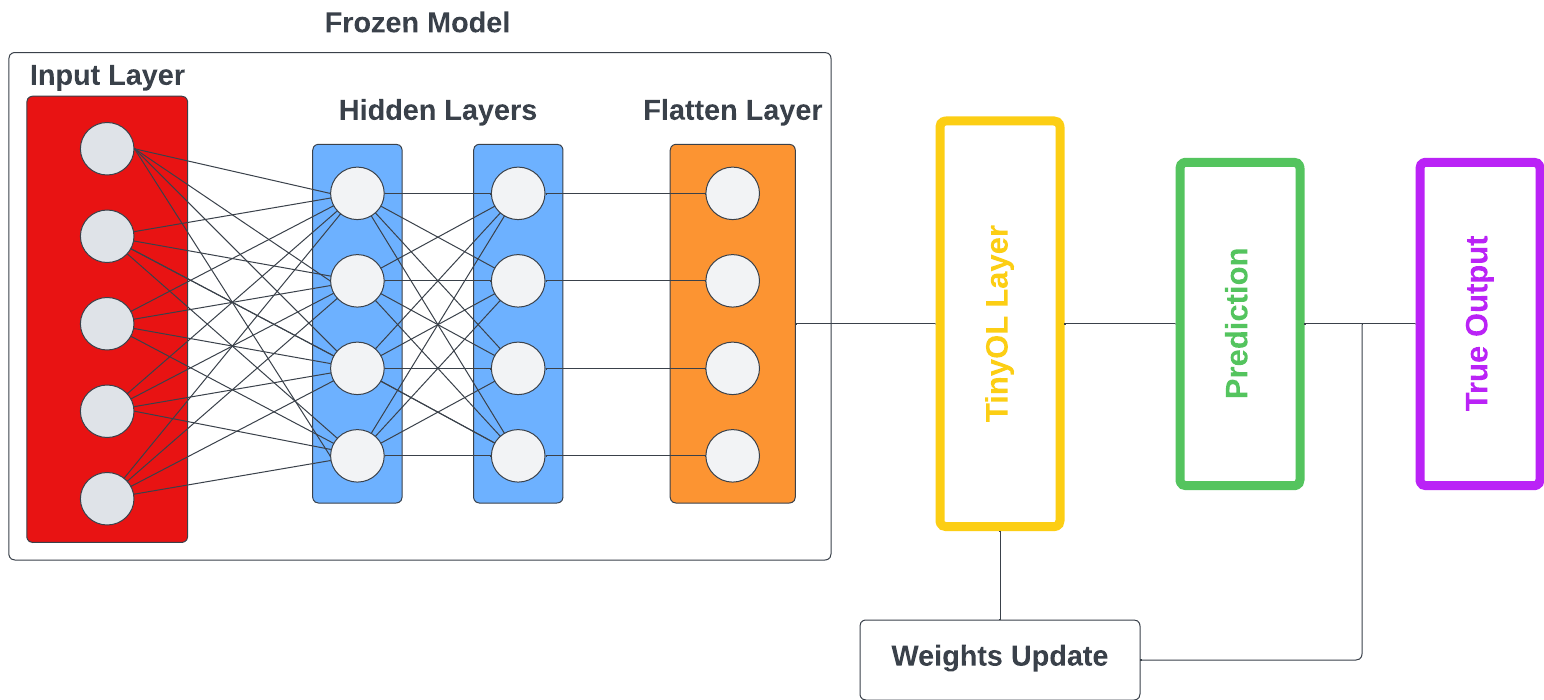
\psfig{file=Images/TinyOL_Machine_learning_network_model.png,width=0.9\textwidth}}
\caption{TinyOL workflow}
\label{OL_network}
\end{figure}

\section{Hardware}
\label{cha:hwardware}
\quad This work employs the MAX78000 \cite{Max78000}, a new breed of AI microcontroller built to enable neural networks to execute at ultra-low power and live at the edge of IoT. It has a feature that makes it stand out among the others: the hardware-based convolutional neural network (CNN) accelerator that enables battery-powered applications to execute AI inferences while spending only microjoules of energy. The accelerator is a perfect solution for TinyML applications thanks to its low energy consumption and the capabilities of running inferences in a short time. 

\begin{figure}[!ht]
\centerline{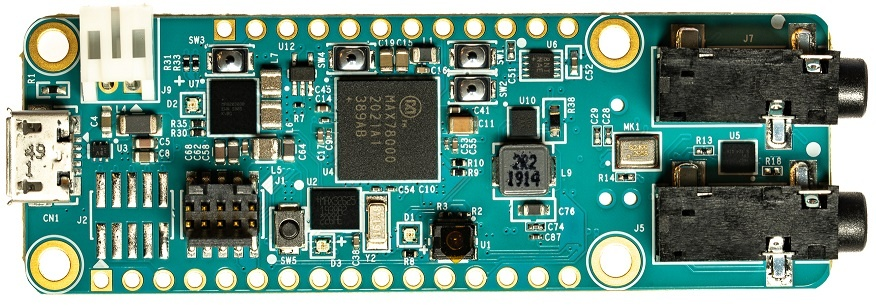
\psfig{file=Images/max78000fthr.jpg,width=0.8\textwidth}}
\setcaptioncitation{https://www.maximintegrated.com/en/products/microcontrollers/MAX78000.html}
\caption{Max78000 FTHR board}
\label{max78000_board}
\end{figure}

\section{CNN Accelerator}
\label{sec:456}
\quad The CNN accelerator consists of 64 parallel processors with 512KB of SRAM-based storage. Each processor includes a pooling unit and a convolutional engine with dedicated weight memory. Four processors share one data memory. These are further organized into groups of 16 processors that share common controls. A group of 16 processors operates as a slave to another group or independently. Data is read from SRAM associated with each processor and written to any data memory located within the accelerator. Any given processor has visibility of its dedicated weight memory and the Data memory instance it shares with the three others.
The CNN accelerator has multiple processors and it was fundamental to understand its functioning and its weights distribution in order to be able to implement a CL model.

%\begin{figure}[!ht]
%\centerline{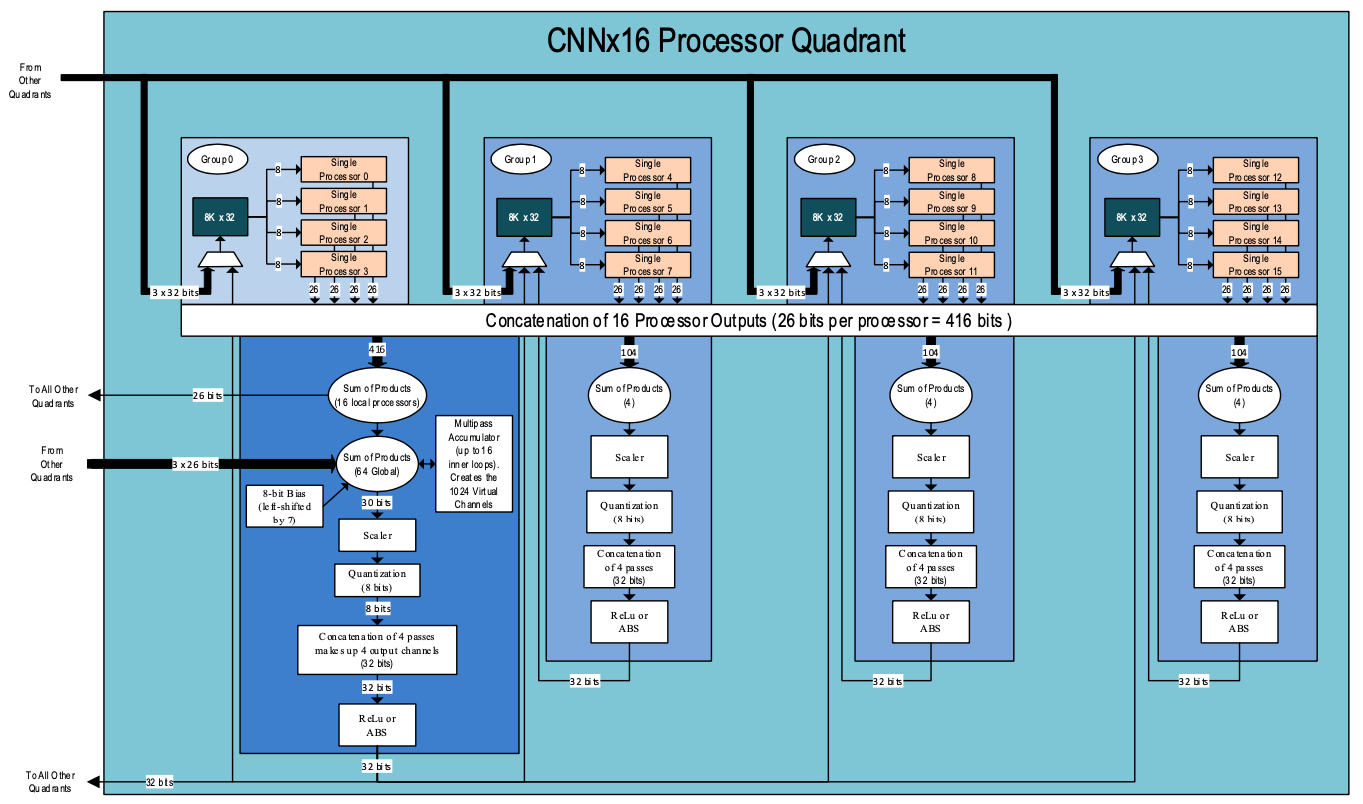
\psfig{file=CNN_accelerator_structure.png,width=0.%9\textwidth}}
%\caption{A quadrant of a CNN accelerator structure}
%\label{cnn_accelerator_structure}
%\end{figure}

\section{CNN model}
\label{sec:457}
\quad The CNN model used in this paper is a five-layer model composed of four convolutional layers with MaxPool and AvgPool and a last linear layer, followed by a Softmax function that extract the percentage of each class. 
The first layer gets an input matrix of 28x28x1, which is an image from Mnist dataset or Emnist dataset. Following, the matrix is convoluted and pooled to obtain a smaller one used to compute the next steps. 
In the end, there is the only one layer that uses biases, all of which are added at each output of the last neurons. 
Each layer uses an activation function named ReLU function, seen in figure \ref{relu}. This function is necessary to map every number into zero if less than zero or from 0 to 127 if greater than zero.

\begin{figure}[!ht]
\centerline{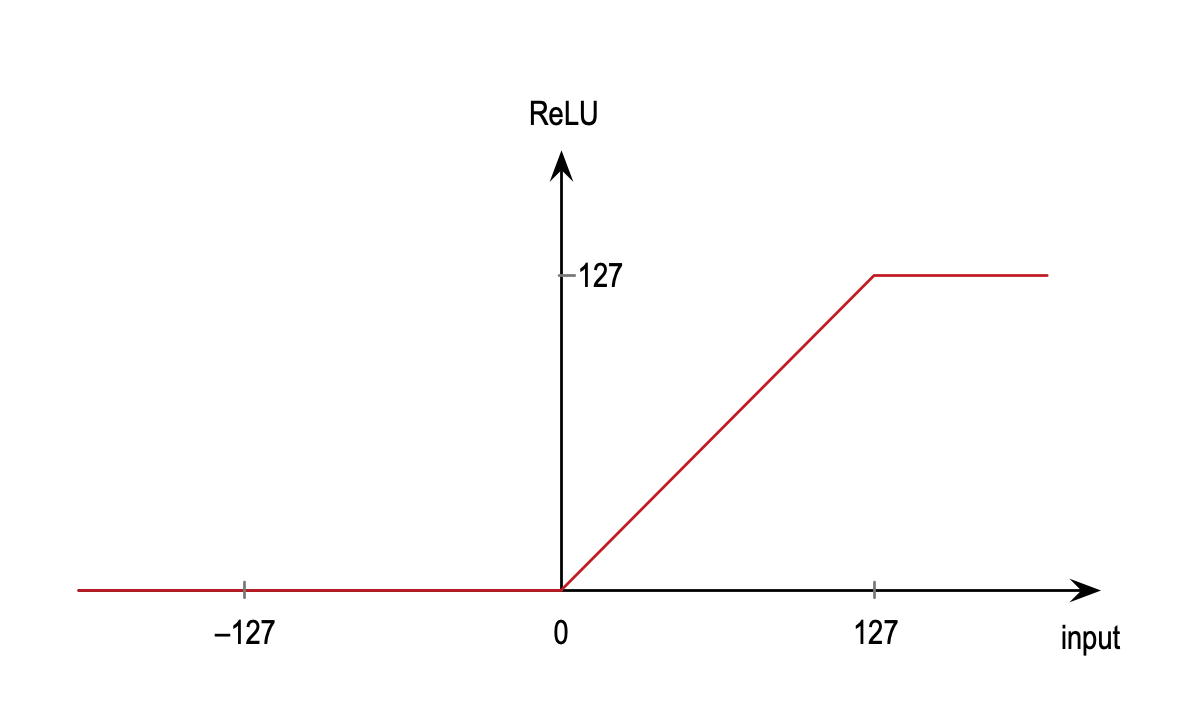
\psfig{file=Images/relu.png,width=0.6\textwidth}}
\setcaptioncitation{https://github.com/MaximIntegratedAI/ai8x-synthesis/blob/develop/docs/relu.png}
\caption{Max78000 relu function}
\label{relu}
\end{figure}

\clearpage
\newpage
\mbox{~}
\clearpage
\newpage
      \chapter{System Implementation}
\label{cha:system_implementation}
\quad Continual Learning is the application of a system capable of self-adjustment and able to learn from incoming data streams. The main competence of this system is indeed the ability to modify weights and biases to learn from the environment and continue to be accurate and reliable for the application. This thesis developed an easier CL system that has to replace a class with another one. In particular the Mnist \cite{deng2012mnist} class 0 will be replaced with a letter from the Emnist \cite{cohen2017emnist} dataset.

\section{Creation of the project}
\label{sec:creation_of_project}
\quad To modify weights and biases it is necessary to know how those values are structured and used. The CNN accelerator uses biases and weights after they are uploaded to memory, which is performed by functions automatically generated with the Software Development Kit (SDK) \cite{SDK}. This series of tools help the developers in many ways. The workflow consists of the first creation and training of a Neural Network model made by specific layers \cite{ai8x-training}. 
Afterward is the synthesis of the model \cite{ai8x-synthesis} , which creates C code that programs the MAX78000 for embedded execution. The program that synthesizes the model needs three inputs a quantized checkpoint file that holds the network weights, a YAML description of the network, and a numpy pickle file with sample input. The code generated by the synthesizer contains a log file that has valuable information about the Networks, which are the kernel map and the values used by each layer divided by processors. The kernel map is a chart 64x768 that shows which kernels are used by each layer. This work focuses on the last layer which uses the first 12 kernels. Furthermore, the layer values are written in layer order, the first row of each processor corresponds to the first output, and so on. These values correspond to the values of the kernel.

\section{Weights allocation}
\label{sec:weights_allocation}
\quad A kernel map is a useful tool needed to understand the order in which each weight is loaded in the memory and then convolute with the output from previous layers. To figure out the sequence of values is fundamental to compare the kernel file and the log file, in particular, each layer and processor with the correspondent kernel. Foremost, upon careful analysis, it is possible to notice that the Kernels are split into 12 portions. At the same time, in the log file, it is possible to observe that the processors are 12 and they are broken up into 10 channels (output neurons). Since there are 12 processors with 10 channels individually and 12 Kernels, it can be inferred that:

\begin{gather*}
    Kernel_j = \sum_{i=0}^{n}\sum_{j=0}^{m} Channel_{i,j}
\end{gather*}

\quad Where $n$ is the number of channels, $i$ is the $i$-$th$ channel, $m$ is the number of processors, and $j$ is the $j$-$th$ processor. 
Each channel piece represents the values of the weights related to their kernel, as seen in figure \ref{weights_allocation}. The bottom line is that every first channel of each processor corresponds to the first output class, the second channel to the second output class, and so forth. 

\begin{figure}[!ht]
\centerline{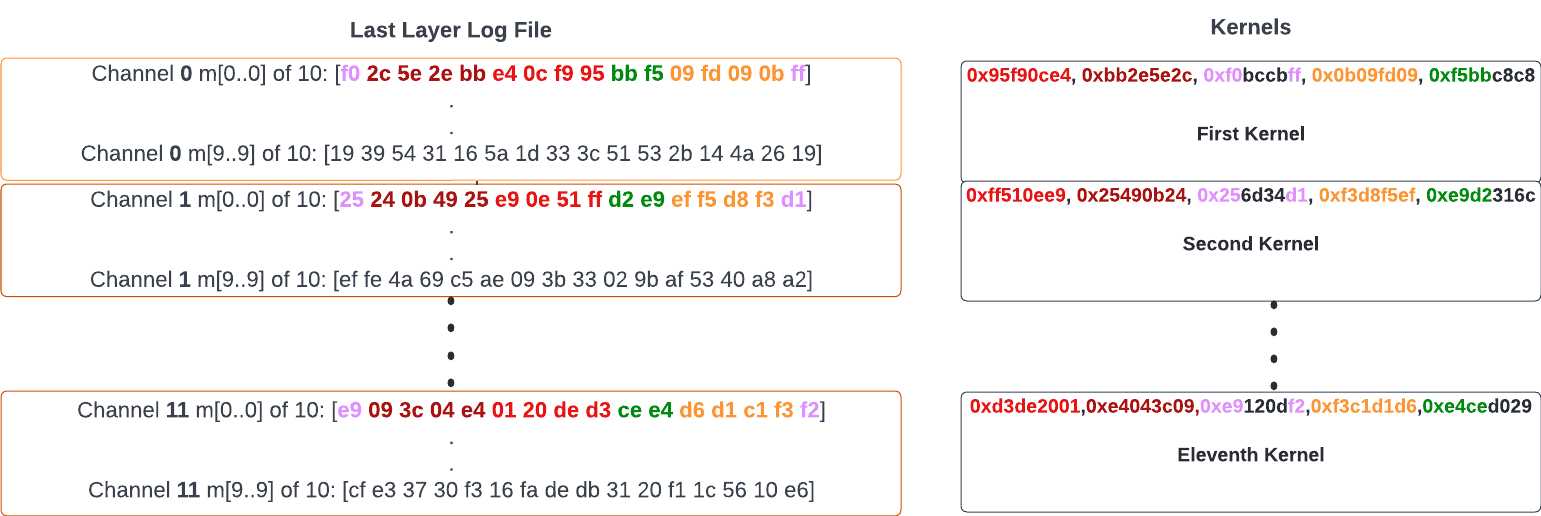
\psfig{file=Images/channel_weigths.png,width=0.9\textwidth}}
\caption{Channels of the last layer together with their correspondent place in the Kernels array}
\label{weights_allocation}
\end{figure}

\section{Last Layer Operation}
\label{sec:last_layer_operation}
\quad Continual Learning bases its functionality on weights update. To perform this operation it is necessary to know the network output with some input. So the first update happens after a complete inference. Since inferences take place inside the hardware-based accelerator, the only way to find out the output of each channel is to multiply the last but one layer output from the CNN accelerator by the weights of channels. This operation is needed because it's hard to find the single output of each channel directly inside the accelerator memory. A solution is to load each layer in succession in the memory, stop the inference at the penultimate layer and unload the result of it. The unload operation consists of a copy of values from specific memory areas. In this case study, the output of the frozen layer is flattened, and thanks to it and the weights from each channel, now it is possible to find the predictions needed for the update. The following chapters will discuss the implementation of the CL system. 

\begin{figure}[!ht]
\centerline{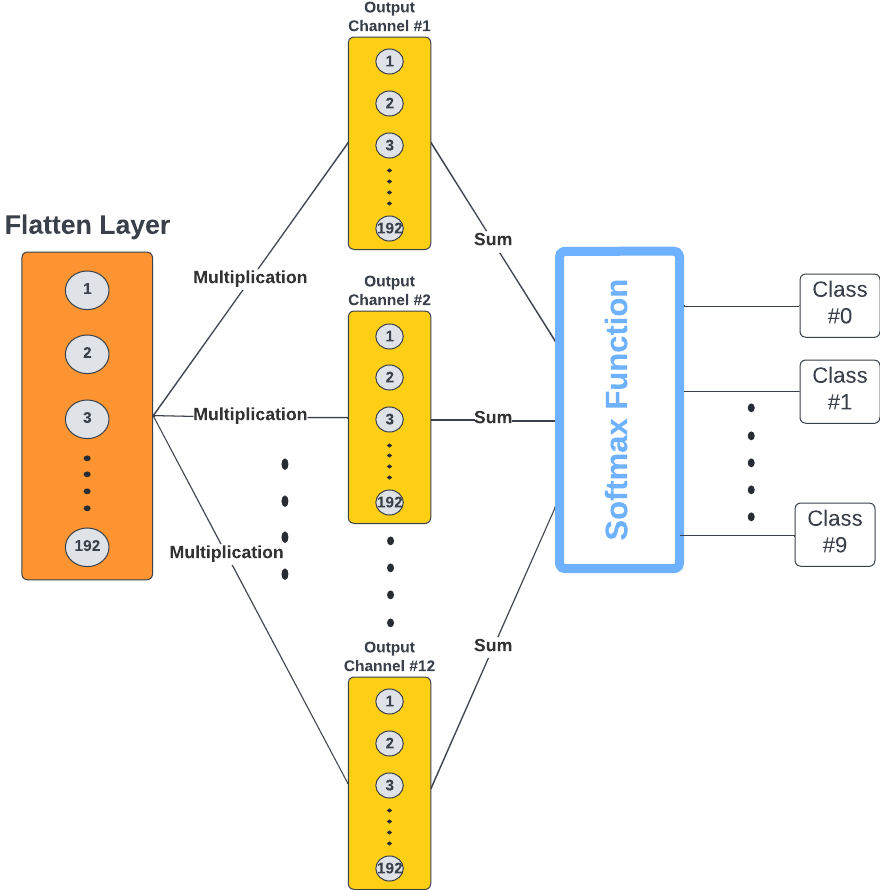
\psfig{file=Images/last_layer_weights_multiplication.png,width=0.6\textwidth}}
\caption{Flattened Layer multiplied by each kernels of last layer and then passed to Softmax Function to obtain percentage of each class}
\label{last_layer_per_weights}
\end{figure}

\section{Continual Learning System}
\label{cha:cl_system}
\quad Continual Learning (CL) is the application of real-time training to generate self-adjusting systems that can learn from never-seen Data. As mentioned in \autoref{sec:CL}, the main feature of CL is the ability of ML models to modify weights and biases to adapt to the environment and be accurate and longstanding reliable. However, CL models on MCU are a new idea that has been barely exploited in recent years. CL applications are not new to the ML scenery, but their function on tiny devices is a new approach. In this thesis, it is developed a similar CL system to the one proposed in \cite{Comprarison_of_Continual_learning_algorithm}. The paper analyses a comparison between different CL algorithm strategies regarding image classification and gesture recognition. The goal is to use a NN model to recognize letters written in the air through data recorded by an accelerometer sensor. The CL strategy is applied only to the last layer of the model, which is added to the pre-trained model and is trained every time a new sample is received.
The idea developed in this thesis started from the implementation of a similar system. The system allows a CNN model to perform continual learning, specifically for classification problems. In this implementation, the CL system is connected to the last layer, which substitutes one class with a not known one. The following section will explain the essential pipeline, and the implemented algorithm.
 
\section{Main pipeline of CL system}
\label{sec:main_pipeline}
\quad TinyML applications are built to be efficient and fast. To apply CL training on embedded devices, it is necessary to develop from scratch a framework that permits the implementation of the CL strategy. The framework is built around the Mnist project template using the same network and the same weights. The system involves the last layer of the network. It aims to enhance the classification abilities of the model, allowing the fine-tune and update of the classification weights and biases, which, over time, lead to better-performing models. The system is a supervised learning application. At every training step, the image fed to the system is class-known. In particular, this study replaces the digit 0 class with the letter A. 
\quad The basic idea of the developed system is to refresh and update the weights every time a new sample is received. This operation can be performed by implementing the standard ML training strategy, which consists of computing the prediction error and propagating it back to the weights. The update to apply depends directly on the impact the specific weights and biases have on the prediction outcome. Once this knowledge is available, it is possible to compute a feedback rule that allows finding the weights that better optimes the loss function. This study applies a CL application to a classification problem. Typically CNN models apply a Softmax activation function to the results of the classifications. This function is fundamental in this system because it permits obtaining a distribution of percentages. The application of CL in this project wants to train only the last layer, as seen in\ref{CL_pipeline}. The part of the model before the last layer is a black box, also called Frozen Model, which works the same for every inference and input. The update rule requires the Softmax function, the output of the Frozen model, the error between prediction and label, and the loss function. To better understand the update function, see \cite[p.~32]{Comprarison_of_Continual_learning_algorithm}

\begin{figure}[!ht]
\centerline{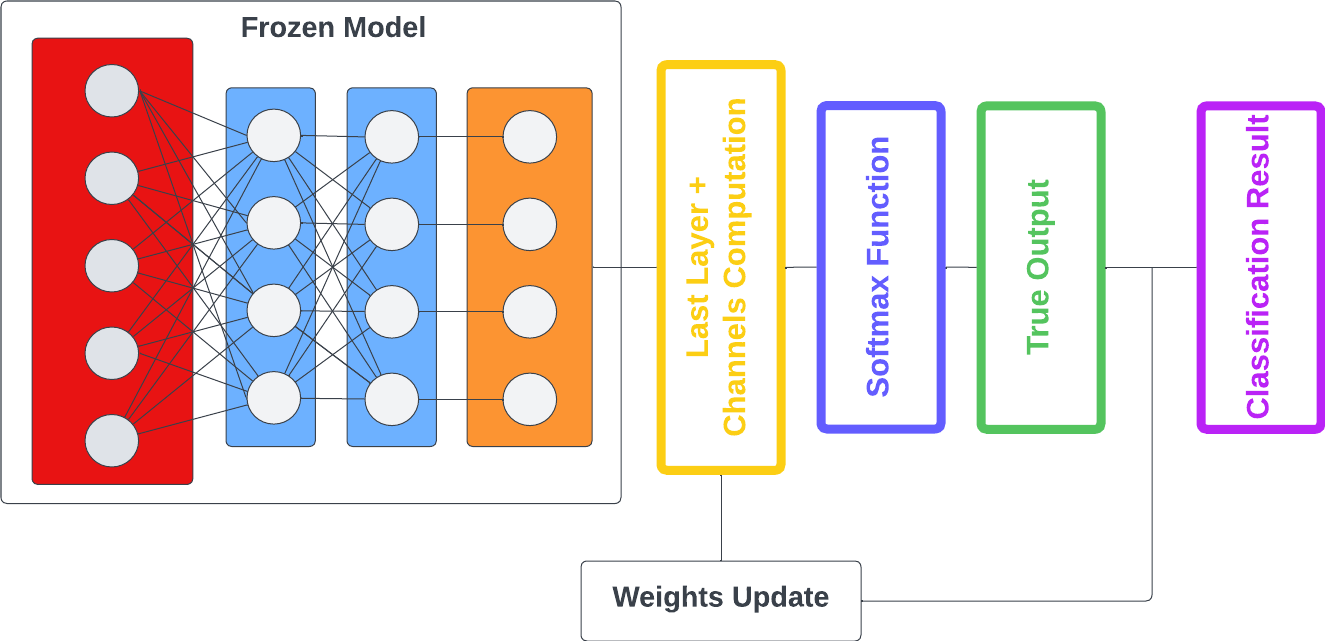
\psfig{file=Images/CL_pipeline.png,width=0.8\textwidth}}
\caption{Basic pipeline of Continual Learning application}
\label{CL_pipeline}
\end{figure}


\section{Implemented algorithm}
\label{sec:ol_alg}

\quad The study implements the TinyOL strategy for performing CL. The TinyOL algorithm is suitable for MCUs thanks to its ease of implementation and management of memories, which is a decisive constraint on embedded devices. The strategy follows the essential ML training step, which consists of computing the error from prediction and propagating it on the weights and biases through stochastic gradients descends (SGD). Its implementation consists of for loops for updating biases and the weights \cite{TinyOl_Paper}. As mentioned in \autoref{sec:weights_allocation}, the key elements that make the implementation complicated, are establishing the allocation of the weights and the rules used by the accelerator to work with them. Initially, the project only updated the weights of the first channel, and by reason of this, slowly, the weights allocation became coherent. Once understood the distribution, the implementation of the strategy could be done. The weights update rule for the TinyOL algorithm are: 


\begin{gather*}
   w_{i,j} = w_{i,j} - \alpha \cdot (y_i - t_i) \cdot x_{i,j} \\
   b_i = b_i - \alpha(y_i - t_i) \\
   where \; i= 0,1..,n \; and \; j = 0,1,..,m
\end{gather*}
 
\quad Where $ y_i $ is the $i$-$th$ value in the prediction array obtained from the Softmax function, $t_i$ is the $i$-$th$ value of the true label array,$x_{i,j}$ is the output of the $i$-$th$ neuron at the $j$-$th$ place, $\alpha$ is the learning rate, $w_{i,j}$ are the weights of the CL layer, $b_i$ are the biases of the CL layer, $i$ is the number of output neurons of the last layer, and $j$ is the height of the last layer of the frozen model. When a new sample is received, the developed CL strategy saves the weights used for the inference in a two-dimensional array. 
\quad Since the weights of each channel are not arranged in the same pattern, another algorithm is needed to update them. As seen in \cite{Continual_Learning_on_Max78000_Microcontroller}, each channel has its approach to using the weights. They use from 5 to 7, 32bit hexadecimal values to extract the weights needed for the computation. Therefore when the update happens, the developed strategy first clips each 32bit hex value into four different 8bit values and then deducts the computed value based on the influence of the weight. The whole algorithm does not work at each iteration, because the update happens just when needed, particularly when the recognition is wrong. Figure \ref{CL_system} contain a diagram showing the TinyOL algorithm.
The method changes the layer parameters at each loop, with no constraints. The model learns from every case received, assuming that the input label and type are correct. This aspect is the main problem that concerns the TinyOL strategy and makes it vulnerable to catastrophic forgetting, a concern from which this model is not protected. This topic is not related to the study proposed in this paper. 

\begin{figure}[!ht]
\centerline{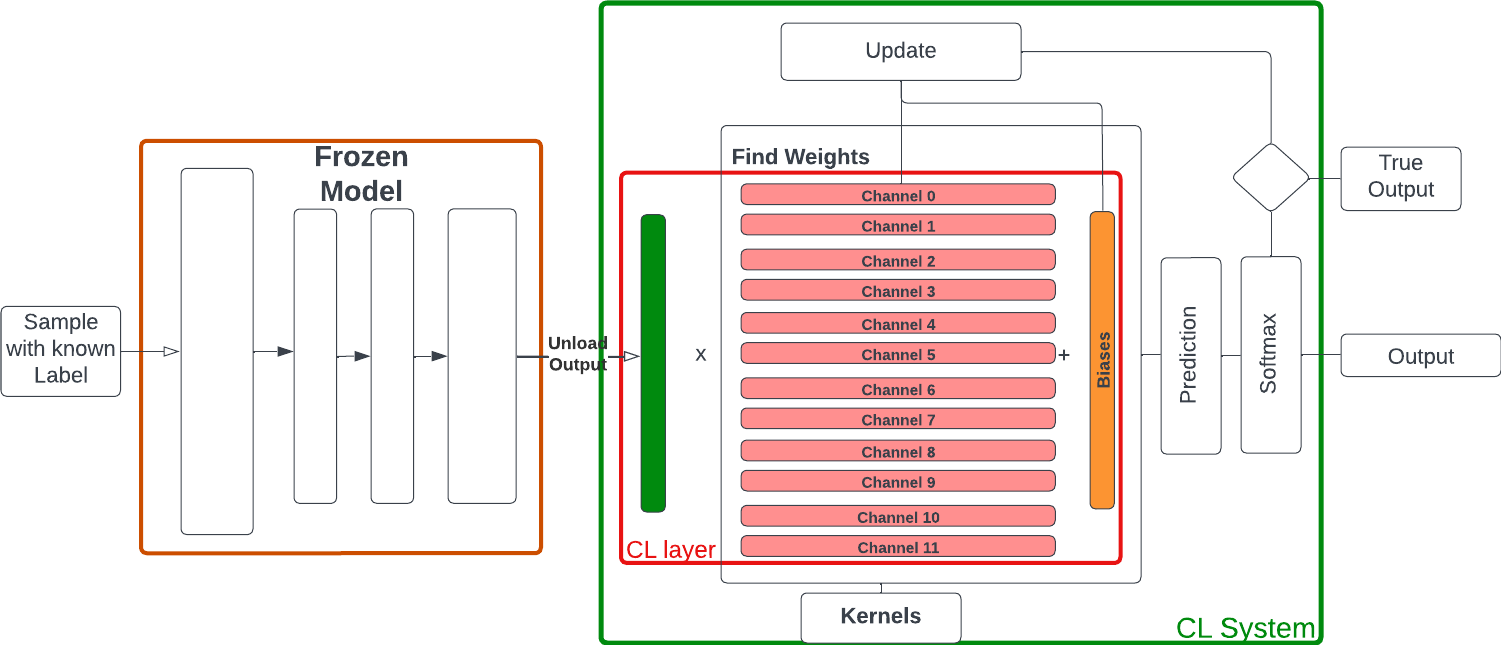
\psfig{file=Images/CL_system.png,width=1\textwidth}}
\caption{Description of TinyOL algorithm on Max78000}
\label{CL_system}
\end{figure}
    



\clearpage
\newpage
\mbox{~}
\clearpage
\newpage


      \chapter{Evaluation}
\label{cha:evaluation}

\quad This chapter describes the practical aspects of the experiments and its results. Initially, the study focused on understanding the theoretical behavior of the methods and the capabilities of CL. Once the requirements stood clear, the focus shifted to the physical project, where with the help of tools \cite{SDK} and as explained in \ref{sec:creation_of_project}, it was possible to understand where to collect the information needed for the CL development. The workflow for the generation of the base template starts with the design of a base model. Then is the training of the classification model based on a Mnist dataset \cite{deng2012mnist} using PyTorch functions adapted to the Maxim tools \cite{ai8x-training}. Afterward is the loading of the network on the embedded device, which is accomplished by the network loader \cite{ai8x-synthesis}. Now is time to collect the new dataset \cite{cohen2017emnist} needed for the CL system to work.

\section{Dataset Collection}
\label{sec:dataset_collection}

\quad This study uses the Emnist dataset. The Emnist dataset is a voluminous publicly available collection of images of hand-written digits having a size of 28 x 28 pixels, specifically the letters collection. It is composed of 145,600 characters balanced in 26 classes. Figure \ref{emnist_example} shows examples of Emnist images. For this study, Python scripts are used to collect the chosen letters 'A' and 'a' from the original dataset. A first conversion is needed from the dataset collection to a NumPy pickle then the synthesizer alters the pickles into samples for the MCU. This transformation is needed because the embedded device uses a characteristic input. After that, another script creates a long array of sample input ready to be used. Due to space constraints, exclusively 40 training samples could be loaded into the memory on the device.  

\begin{figure}[!ht]
\centerline{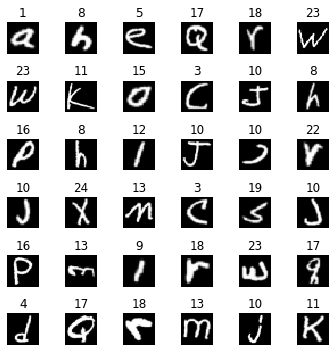
\psfig{file=Images/emnist_examples.png,width=0.6\textwidth}}
\caption{Example of images from Emnist dataset}
\label{emnist_example}
\end{figure}

\section{Network Model}
\label{sec:network_model}

\quad Convolutional Neural Network (CNN) model is the architecture used in this image classification application. Computer vision uses CNN models for the elaboration of images. Its main feature is the presence of convolutional layers for feature extraction. This type of structure allows the ML model to perform initially a feature extraction over the image and to flatten the output matrix to an array. Following is the NN layer for the classification. Figure \ref{input_output_model} represent the structure of the model. The frozen model contains four convolutional layers followed by the ReLU activation function \ref{relu}. The last 3 layers of the frozen model are Max pooled and Avg pooled. The fully connected layer is used to elaborate the array and later feed the data to the classification layer, where the Softmax activation function is used to produce the probability of each class. 

\begin{figure}[!ht]
\centerline{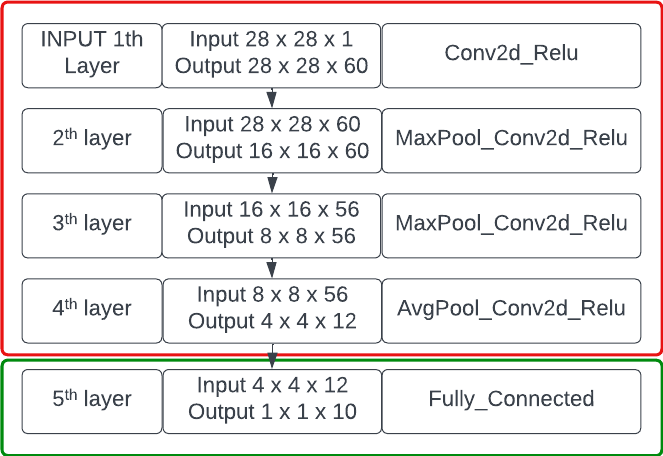
\psfig{file=Images/Input_output_model.png,width=0.6\textwidth}}
\caption{Description of the model. Structure and input-output size. Frozen model in red, and CL layer in green}
\label{input_output_model}
\end{figure}

\section{Model Training}
\label{sec:model_training}

\quad It was possible to obtain the base model through the tools given by Maxim. As said before, the base model is the Mnist network. During the training, it was possible to monitor the progress and performance of the model. This phase was crucial to designing the best-performing network. Figure \ref{training_results} the results of the training over epochs.

\begin{figure}[!ht]
\centering
     \begin{subfigure}[b]{0.4\textwidth}
         \centering
         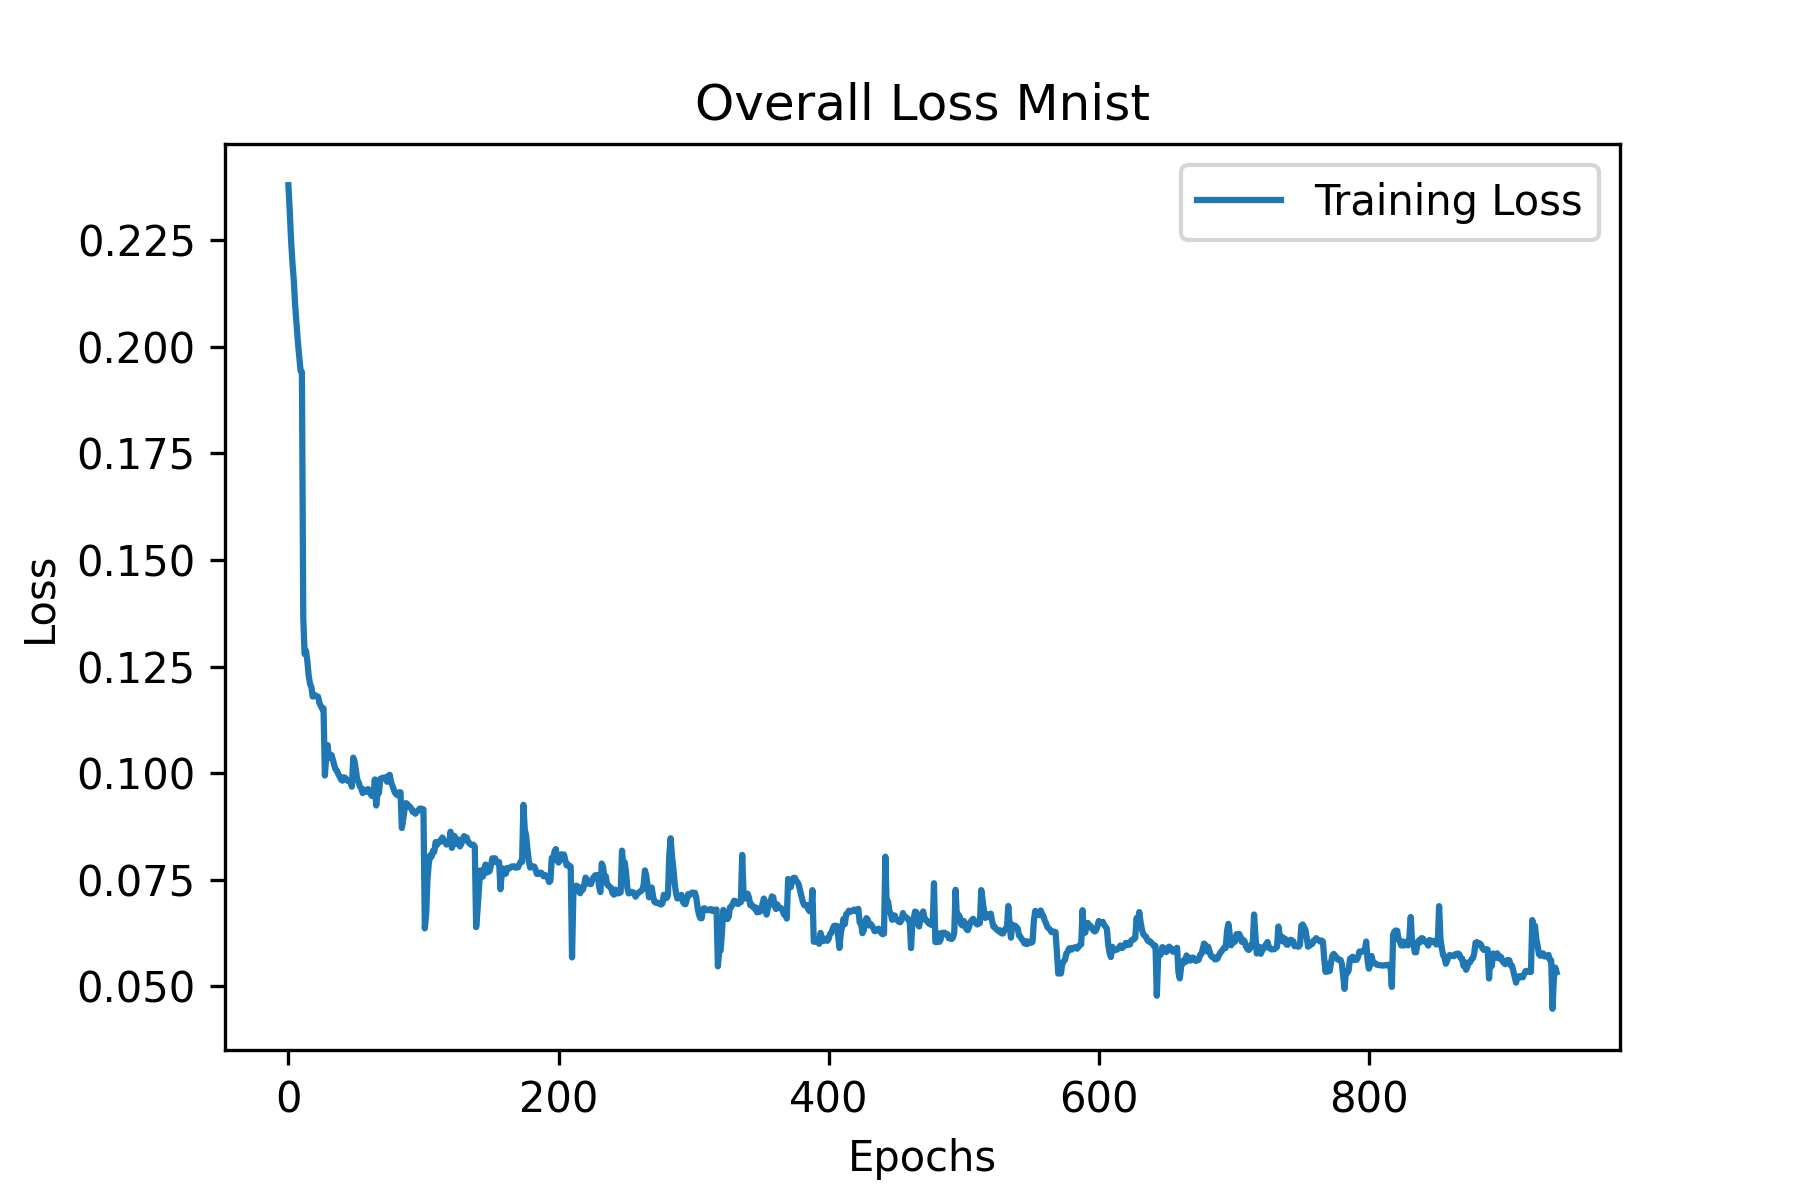
\includegraphics[width=\textwidth]{Images/plot_training_loss_mnist.png}
         \caption{Overall loss of training over time.}
         \label{fig:training_loss}
     \end{subfigure}
     \hfill
     \begin{subfigure}[b]{0.4\textwidth}
         \centering
         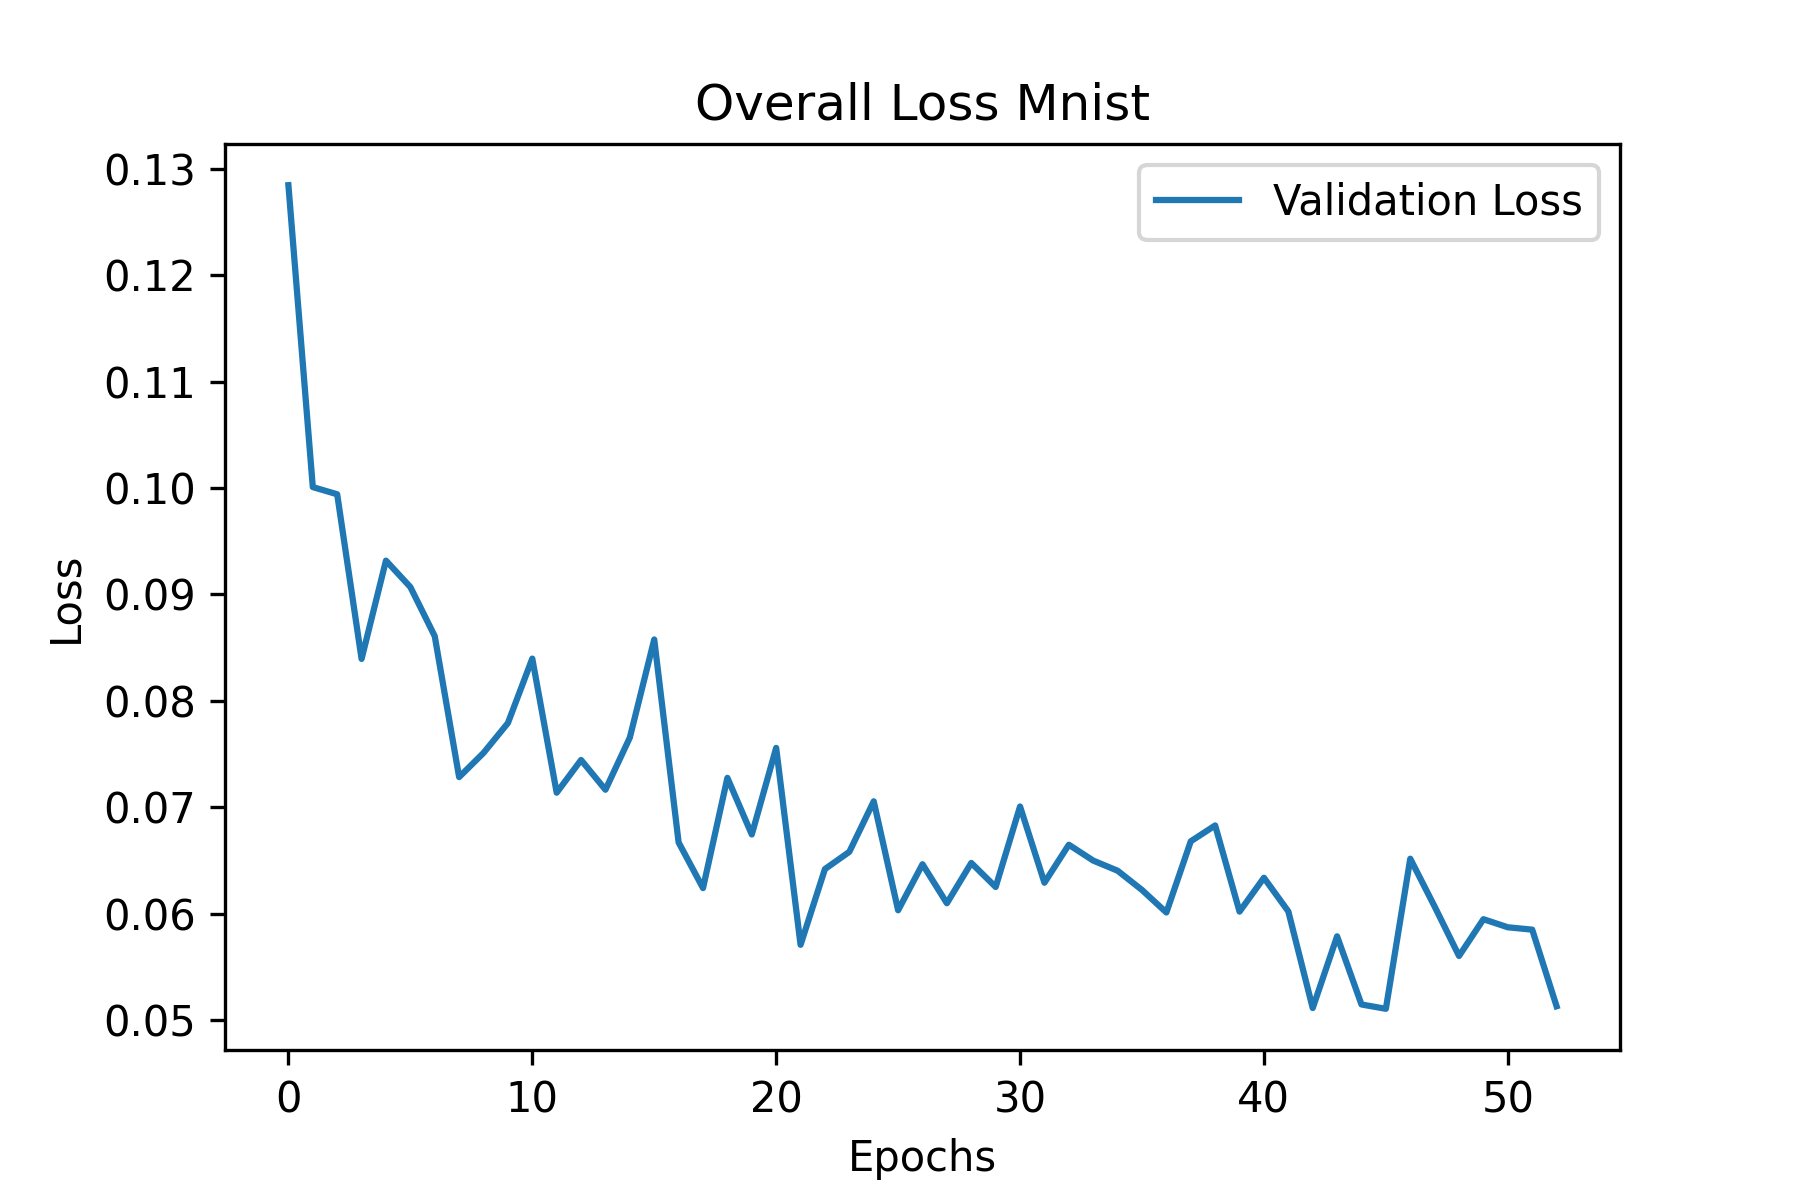
\includegraphics[width=\textwidth]{Images/plot_validation_loss_mnist.png}
         \caption{Overall loss of validation over time.}
         \label{fig:validation_loss}
     \end{subfigure}
     \hfill
     \begin{subfigure}[b]{0.4\textwidth}
         \centering
         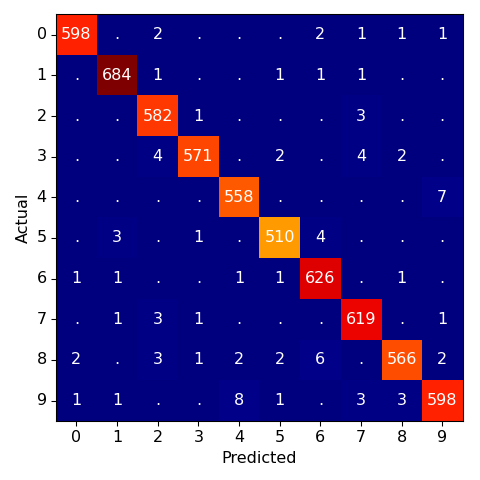
\includegraphics[width=\textwidth]{Images/plot_mnist_confusion_matrix.png}
         \caption{Confusion matrix.}
         \label{fig:confusion_matrix}
     \end{subfigure}
        \caption{Training results of Mnist model training taken with Tensorflow}
        \label{training_results}
\end{figure}

\section{Frozen Model}
\label{sec:frozen_model}

\quad In the embedded device field, memory and speed are key features. Designing the model considering the memory constraint is a fundamental step. Because of this, the model is a tiny example of a Neural Network, composed of 5 layers. In the application, the frozen model is composed of 4 layers, which are used for the feature extraction. Since the images of the two datasets have similar features, this project uses the same frozen model for the two different images. The comparison plot can be seen in \ref{comparison_frozen_model}. 

\begin{figure}[!ht]
\centerline{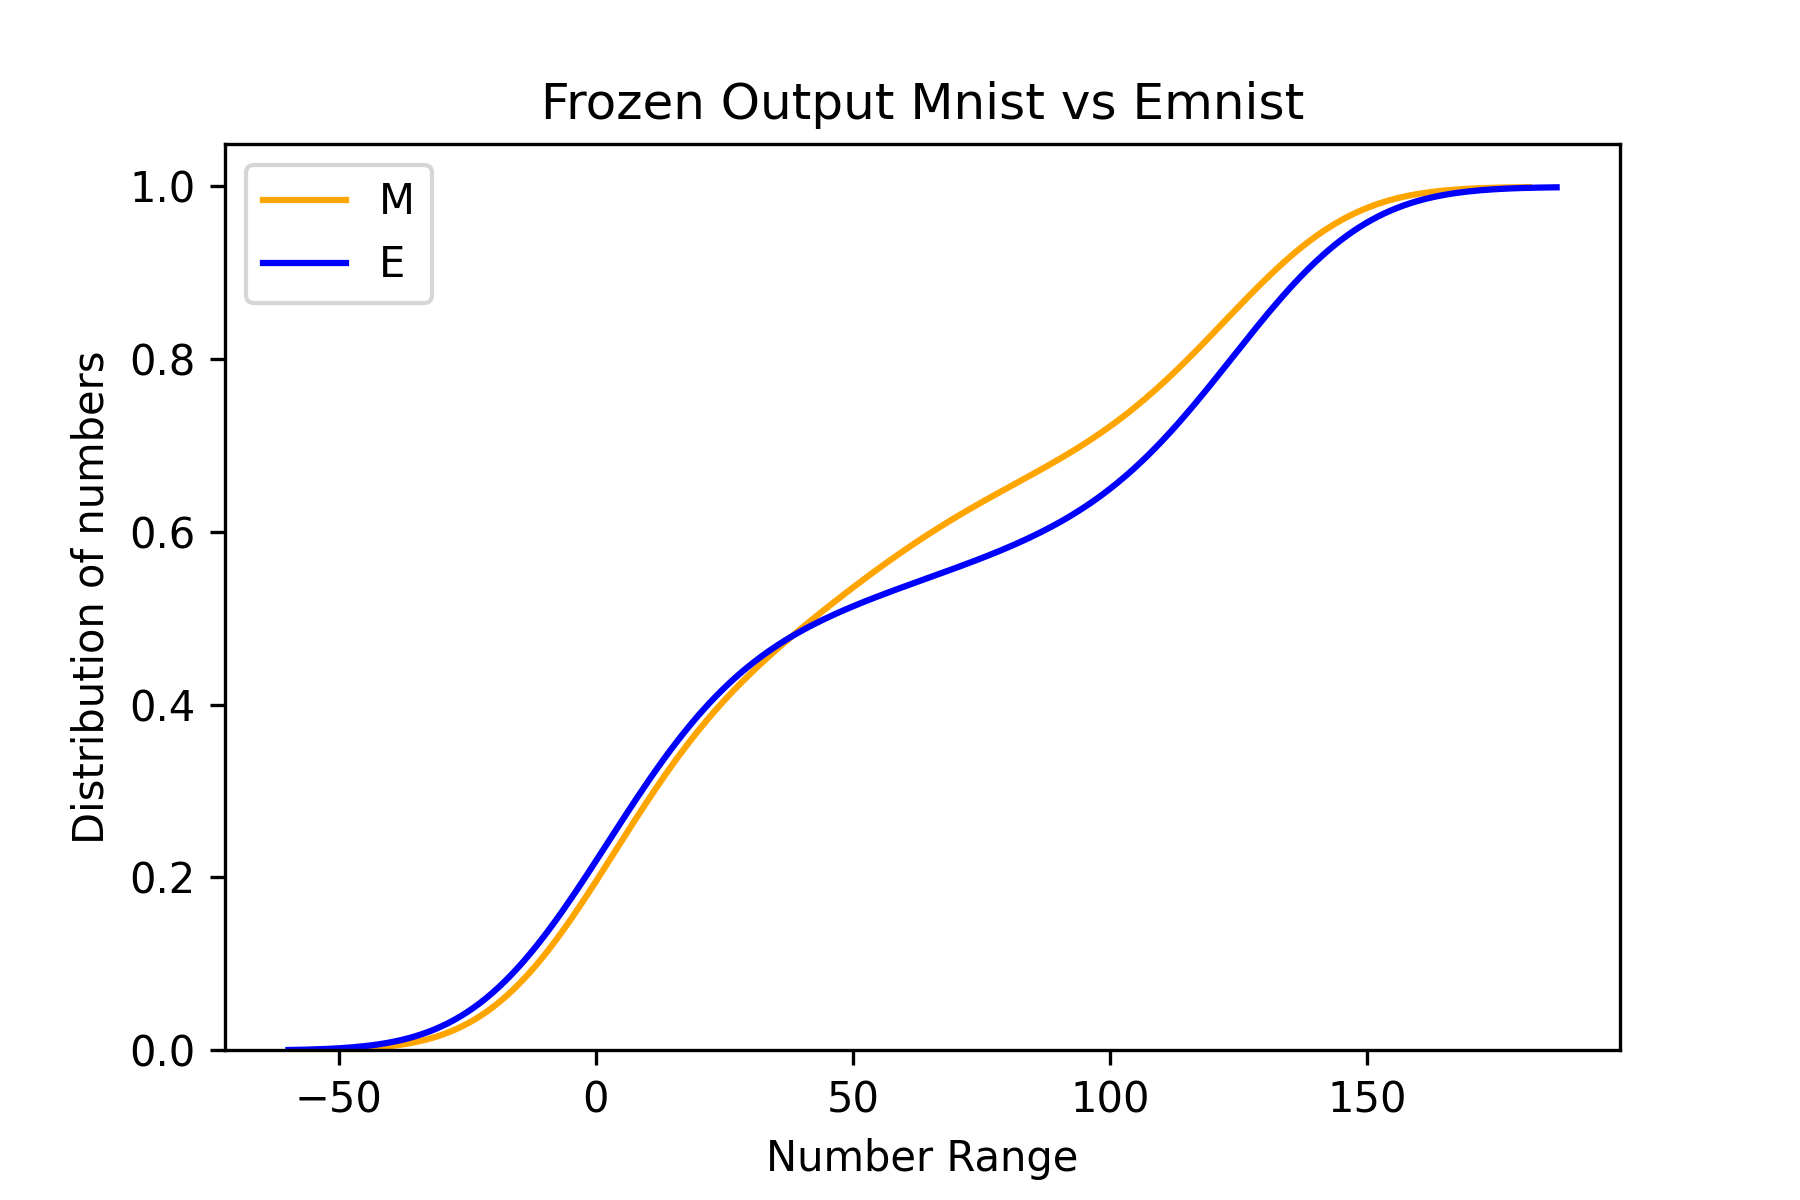
\psfig{file=Images/plot_frozen_model_emnist_mnist.png,width=0.8\textwidth}}
\caption{Comparison of output of feature extractions Mnist vs Emnist}
\label{comparison_frozen_model}
\end{figure}

\section{Max78000 setup}
\label{sec:application_setup}

\quad This section describes the setup needed to run the application correctly and explains each step. First, to deploy the code is necessary to configure the computer as explained in \cite{SDK}, the tools used are OpenOCD and Arm-gdb which allows a connection to the board permitting the flashing of codes. The dataset, model, final layer, and system can all be deployed on the MCU once they are all ready.  Initially, the code set up the board parameters, such as the clock source and the debugger, then it enables the CNN accelerator clock and starts a loop. Each loop is composed like this: first, there is the initialization and the loading of weights biases and inputs, followed by the configuration and inferences of the CNN, during which the output of the frozen layer is captured. Following is the computation of the channel's outputs, which will be used to calculate the update values. In the end is the back-propagation phase, which updates neuron weights and biases according to the Softmax function. When the loop ends, the code computes complete inferences on training and testing samples to correctly classify the system accuracy. Additionally, an inference on a Mnist digit is computed to check if during the CL training the catastrophic forgetting happened.


\section{Experimental Results}
\label{cha:experimental_results}

\quad The next sections describe and discuss all the results of the experiment performed. The system is developed in the MCU, but on the other hand, the experiment's results have been docketed by the MCU itself or an external device. Time and energy consumption are measured with X-NUCLEO-LPM01A \cite{nucleo}. The test has been carried out in a supervised environment, where the sample data are established a priori. The input samples handled are all 'A's taken from the EMNIST dataset. In this way, it was possible to make an ideal model classification. 

\section{Continual Learning on Max78000 Microcontroller}
\label{sec:image_classification}

\quad The aim is to replace the weights and biases of the neuron responsible for recognizing class 0. Specifically, previously this neuron had the task of identifying the digit 0, then because of continual learning, it can recognize the letter A. Due to memory constraints a total of 40 samples have been used to fulfill the training. THe table represented in Figure \ref{time_inferences} shows an overview of times for the frozen model inference and the CL system. In this case the average inference time of the frozen model includes the weights and biases loading, and the initialization and configuration of the CNN accelerator. Different clock sources are applied, and in every case, is preserved the same ratio. Figure \ref{time_single_layer} displays the time that each layer take to perform inference. The clock of the CNN accelerator has a maximum speed of 50 MHz. The hardware-based accelerator computes inferences in a short time. 

\begin{figure}[!ht]
\centerline{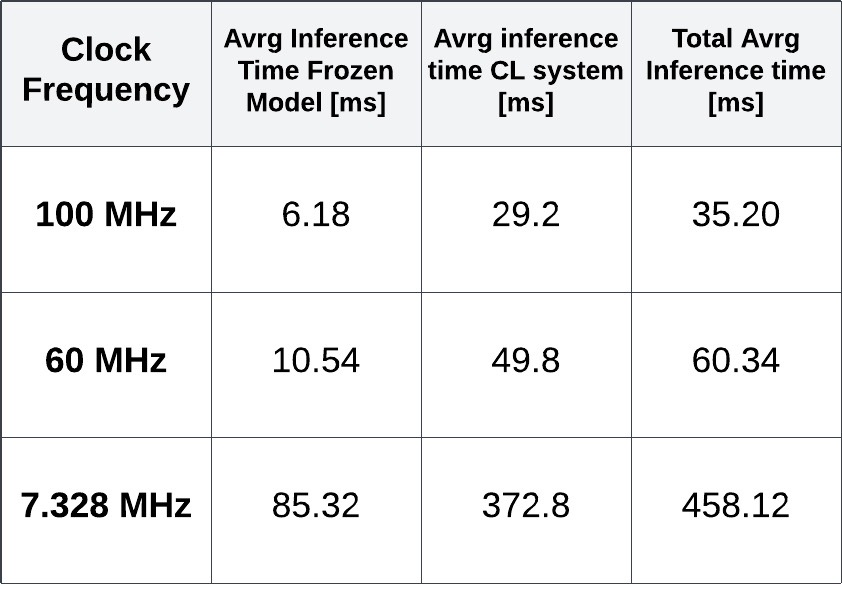
\psfig{file=Images/time_inference_cl_table.png,width=0.8\textwidth}}
\caption{Table comparing the overall time of initialization and inference of frozen model and CL layer with different clock sources.}
\label{time_inferences}
\end{figure}

\begin{figure}[htbp]
\centerline{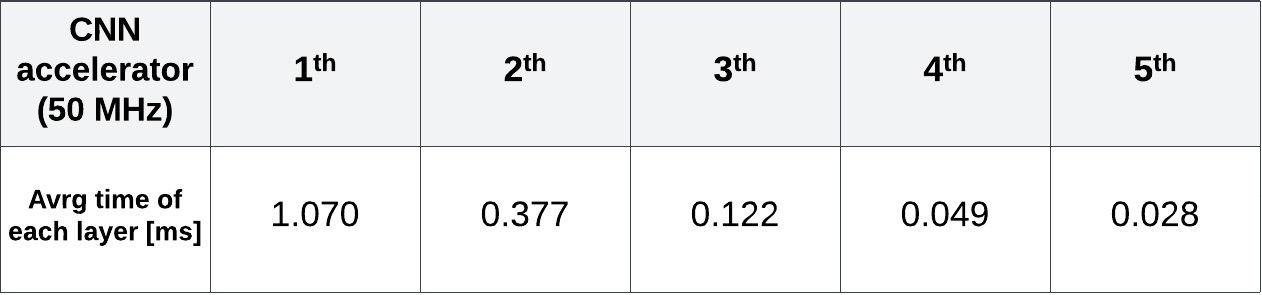
\psfig{file=Images/time_single_layer_inference_cnn.png,width=0.8\textwidth}}
\caption{Table showing time inferences of each layer inside the CNN accelerator.}
\label{time_single_layer}
\end{figure}

\singlespacing

\quad Figure \ref{time_backpropagations_iterations} illustrates two distributions of time needed to apply the back-propagation. The first plot shows the time distribution of 100 iterations, figuring the weights update does not occur at each loop, but it happens just when an update is needed. According to the algorithm, the update occurs just when a classification turns out wrong. It is possible to state that, as seen in the \ref{fig:time_1000_iterations} plot, after some iterations, the update stops to happens because the system adjusted the weights to recognize the new class.

\begin{figure}[!ht]
\centering
     \begin{subfigure}[b]{0.4\textwidth}
         \centering
         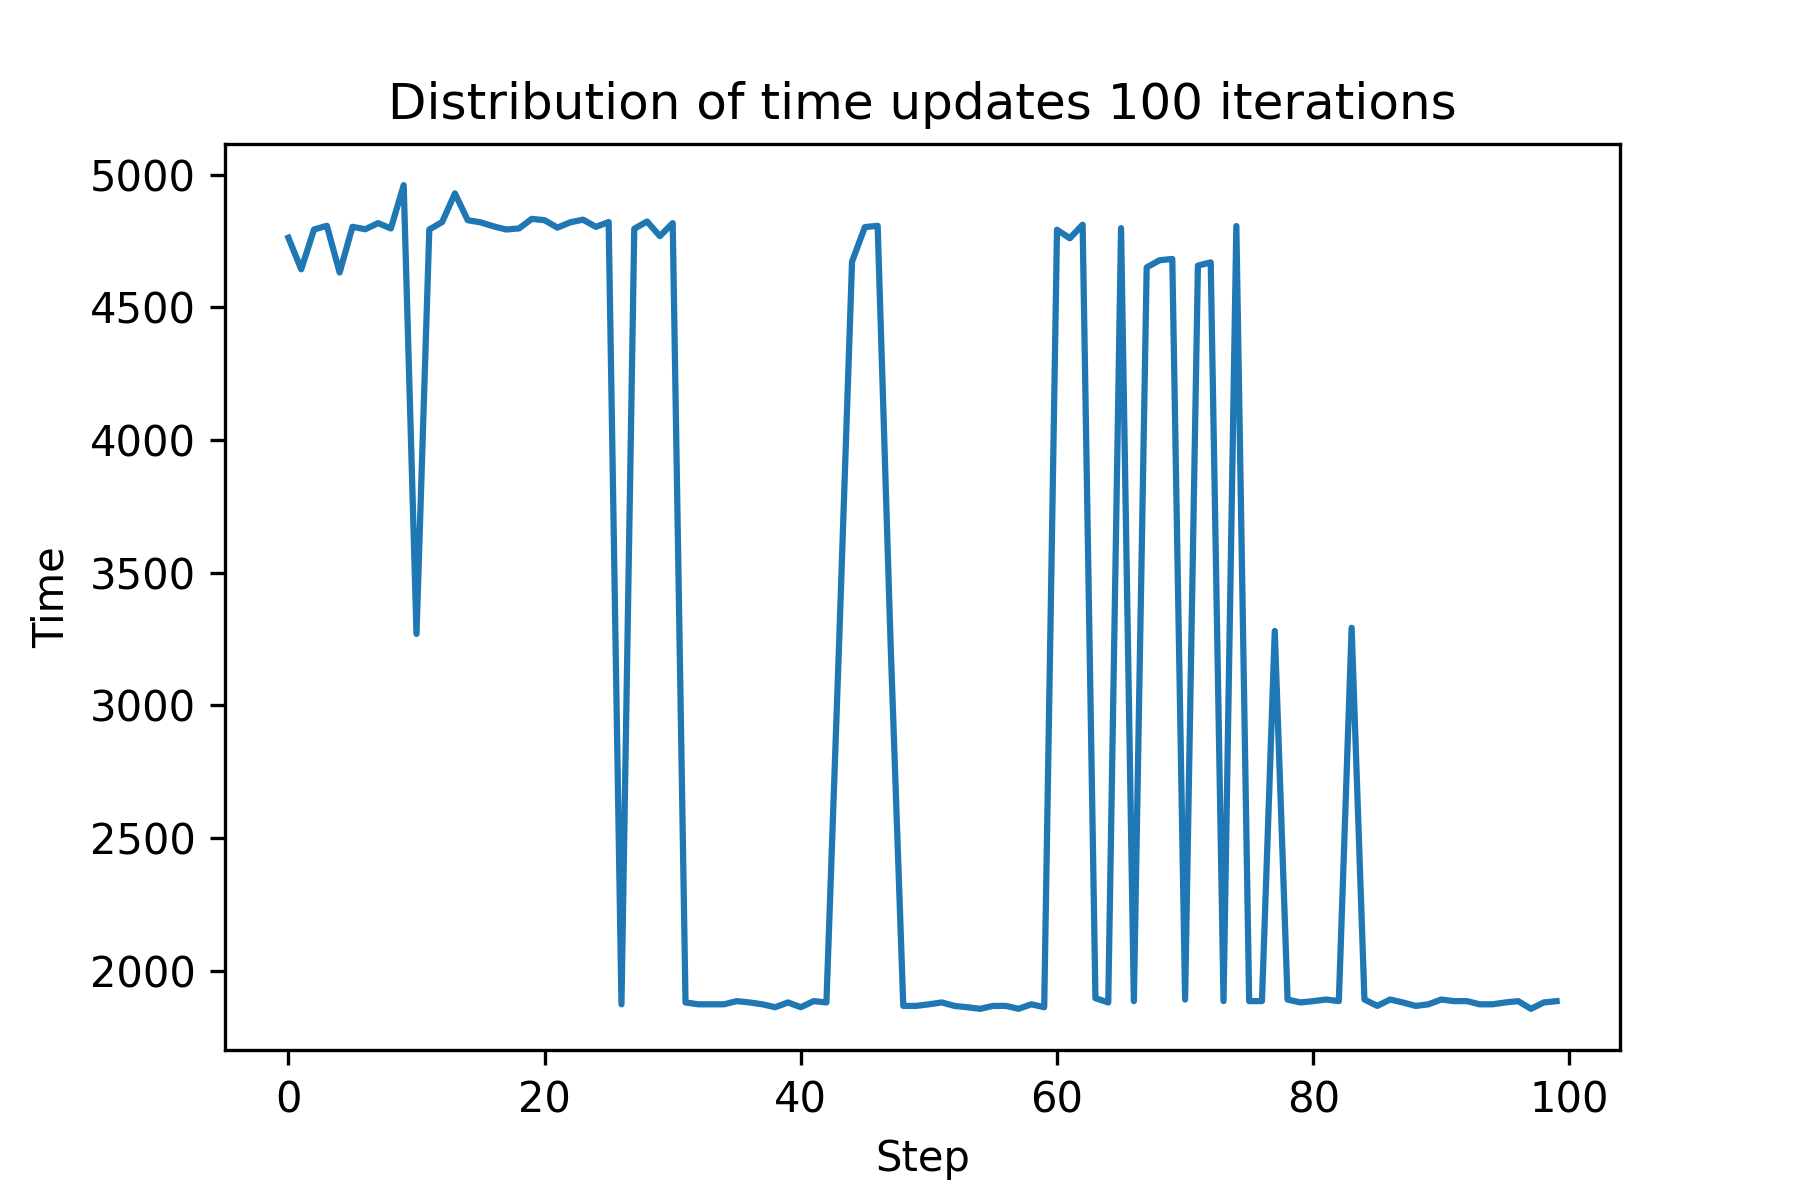
\includegraphics[width=\textwidth]{Images/plot_distribution_time_update_100.png}
         \caption{Plot of backpropagation time for 100 iterations.}
         \label{fig:time_100_iterations}
     \end{subfigure}
     \hfill
     \begin{subfigure}[b]{0.4\textwidth}
         \centering
         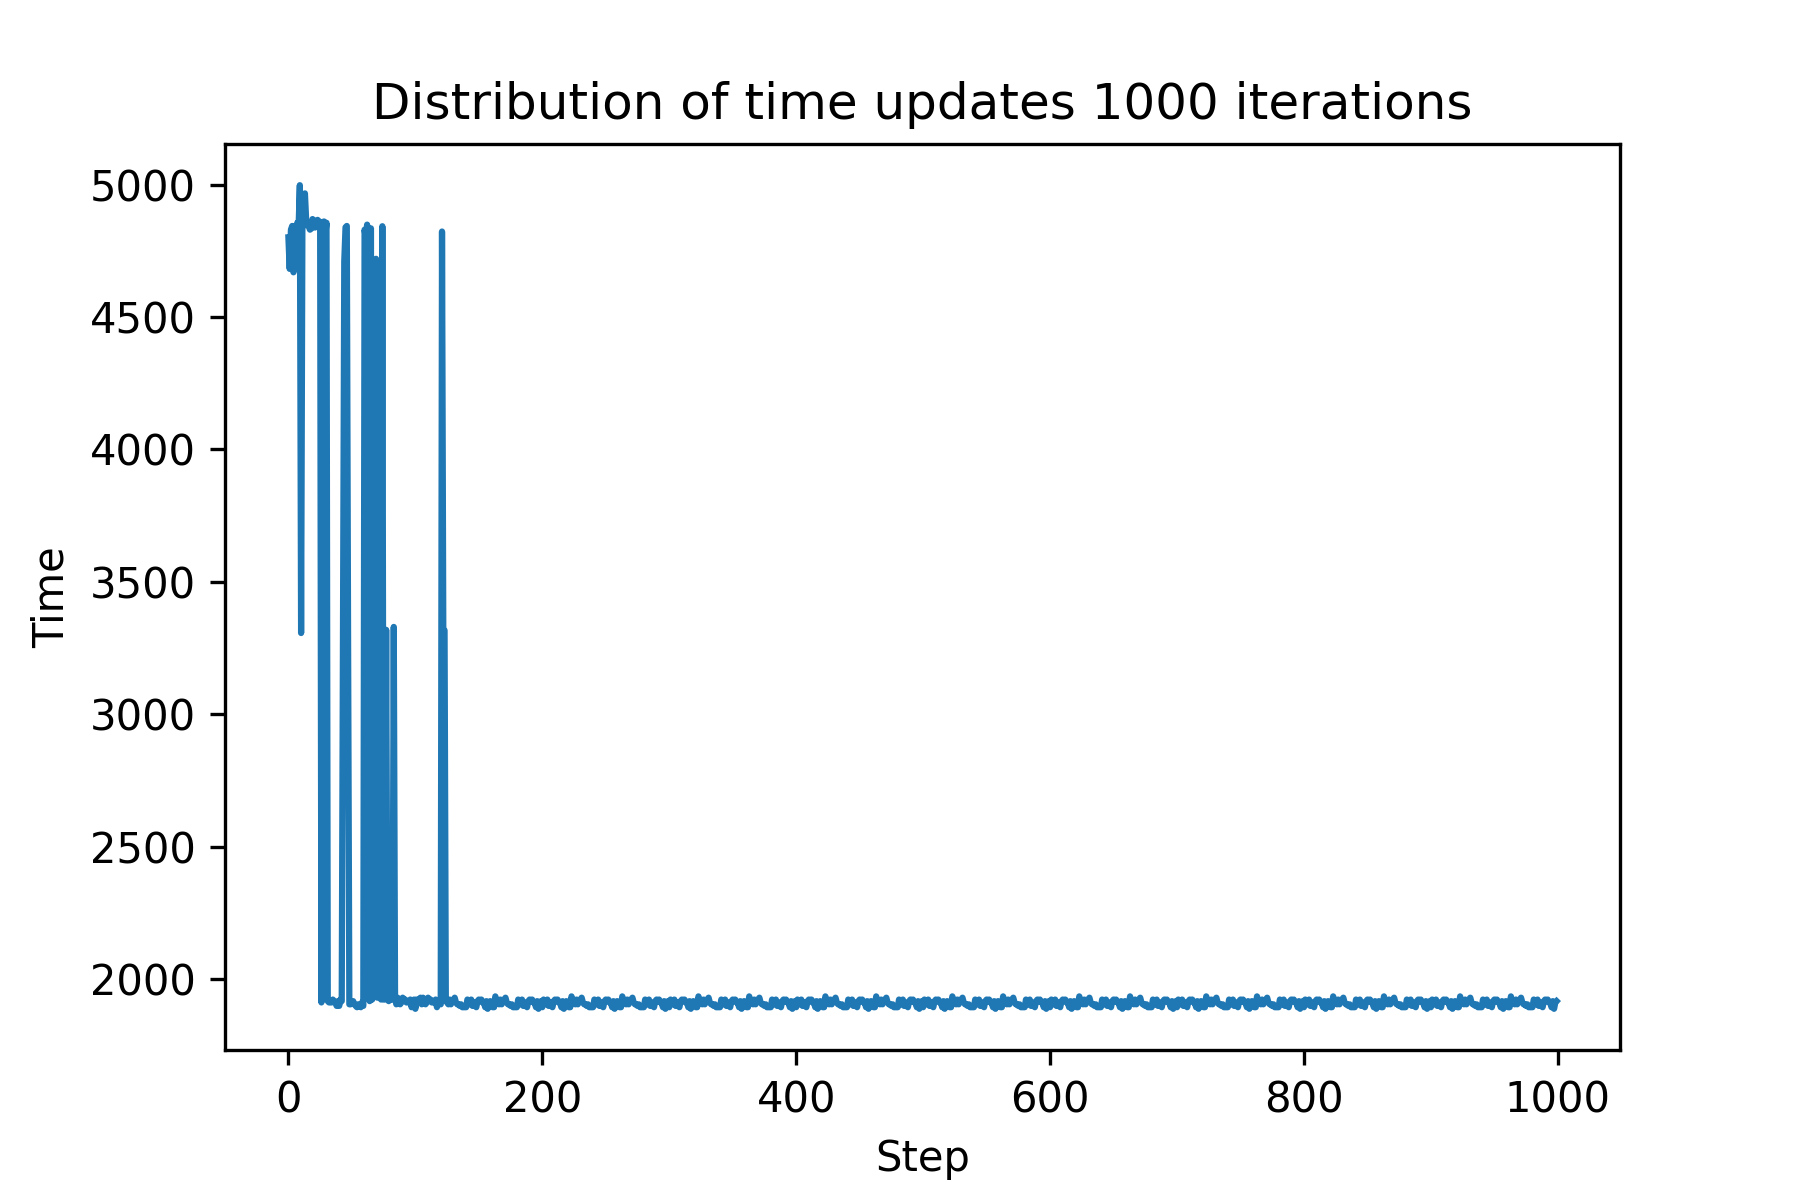
\includegraphics[width=\textwidth]{Images/plot_distribution_time_update_1000.png}
         \caption{Plot of backpropagation time for 1000 iterations.}
         \label{fig:time_1000_iterations}
     \end{subfigure}
     \hfill
        \caption{Distribution of the time that backpropagation takes at each iteration}
        \label{time_backpropagations_iterations}
\end{figure}

\singlespacing

\quad Low energy consumption is a key feature in the MCU field. Table \ref{energy_consume} contains an overview of energy consumption. This table shows the comparison between different clock sources, such as 100 MHz, 60 MHz, and 7.328 MHz. It is possible to state that the average energy consumed by the device is low. It is interesting to notice that the energy consumption at 60 MHz is lower than 100 MHz, but when the clock is reduced drastically to 7.328 MHz, the energy utilization grows exponentially. The clock source is almost fourteen times slower than the fastest, but the energy drained is nearly four times higher. Operations consume less because program execution is slower; on the other hand, the formula 
\begin{gather*}
   Energy = Power \cdot Time
\end{gather*}
\quad implies that proportionally with a longer execution time, there will be equally higher energy consumption.

\begin{figure}[!ht]
\centerline{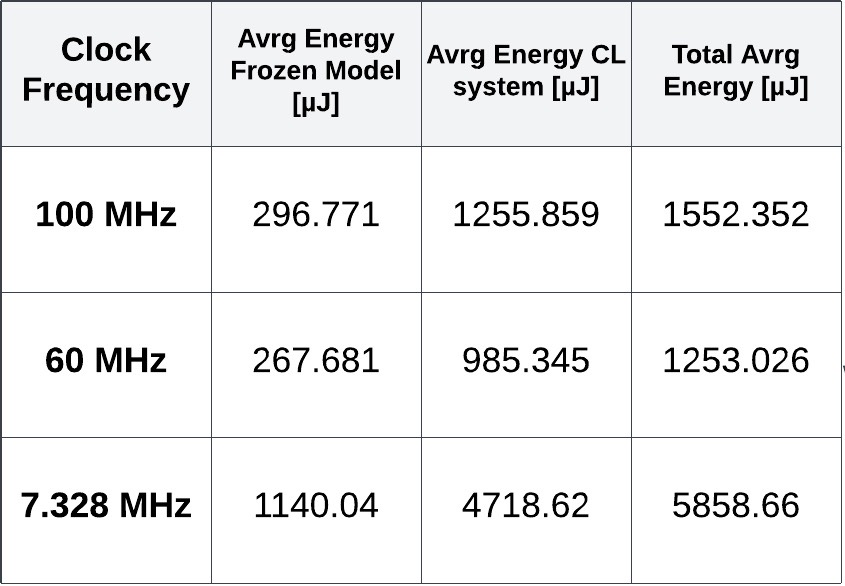
\psfig{file=Images/energy_cnn_cl.png,width=0.8\textwidth}}
\caption{Table showing the energy consumed with different clock source and by CNN and CL system.}
\label{energy_consume}
\end{figure}

\singlespacing

\quad Figure \ref{plot_accuracy} shows the model accuracy over iterations. It is possible to notice that after enough iterations, the model can recognize images more accurately. The plot serves as evidence that the algorithms are reliable and well-implemented. Furthermore, it should be highlighted that this experiment does not show significant catastrophic forgetting. After the algorithm finishes, the program computes an inference on the Mnist dataset resulting in 100\% accuracy on the right class.

\begin{figure}[!ht]
\centering
     \begin{subfigure}[b]{0.4\textwidth}
         \centering
         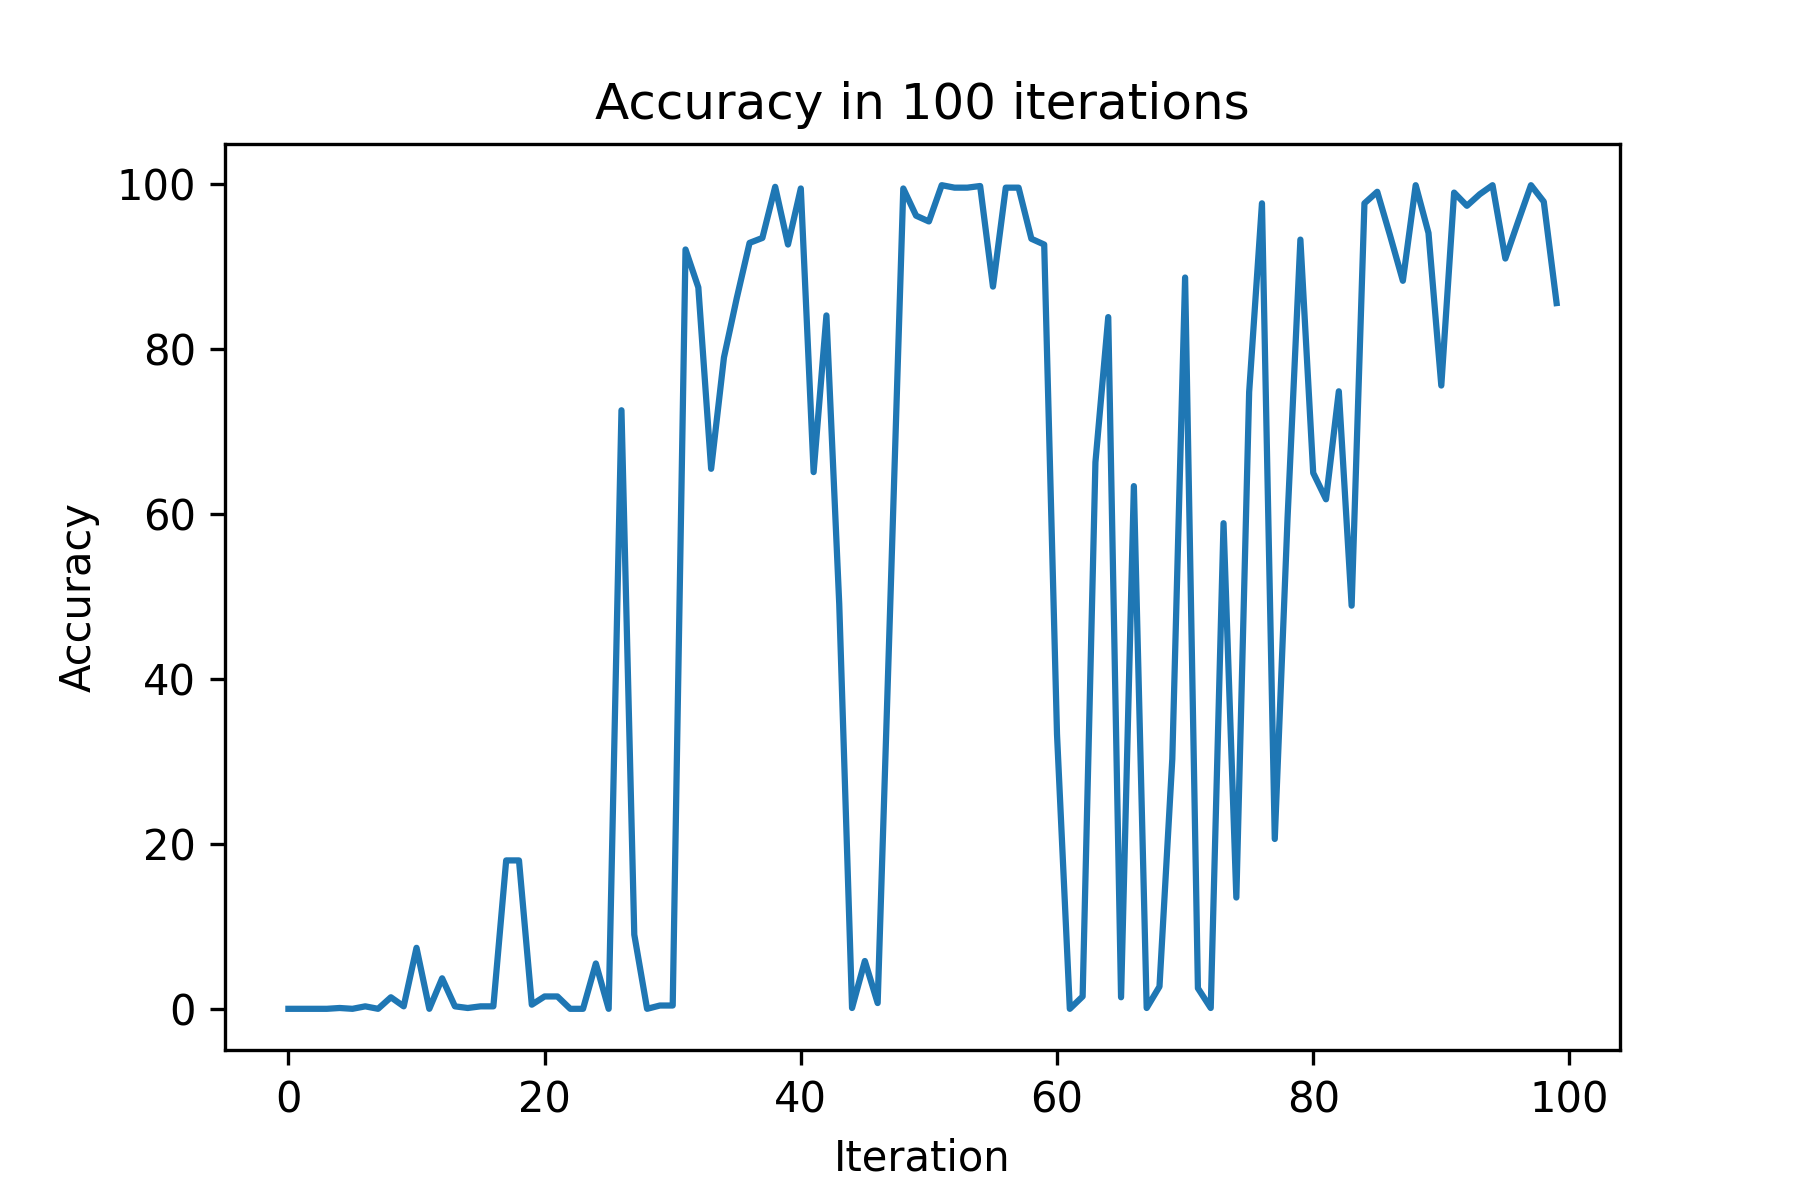
\includegraphics[width=\textwidth]{Images/plot_accuracy_100.png}
         \caption{Plot of accuracy over 100 iterations.}
         \label{fig:accuracy_100}
     \end{subfigure}
     \hfill
     \begin{subfigure}[b]{0.4\textwidth}
         \centering
         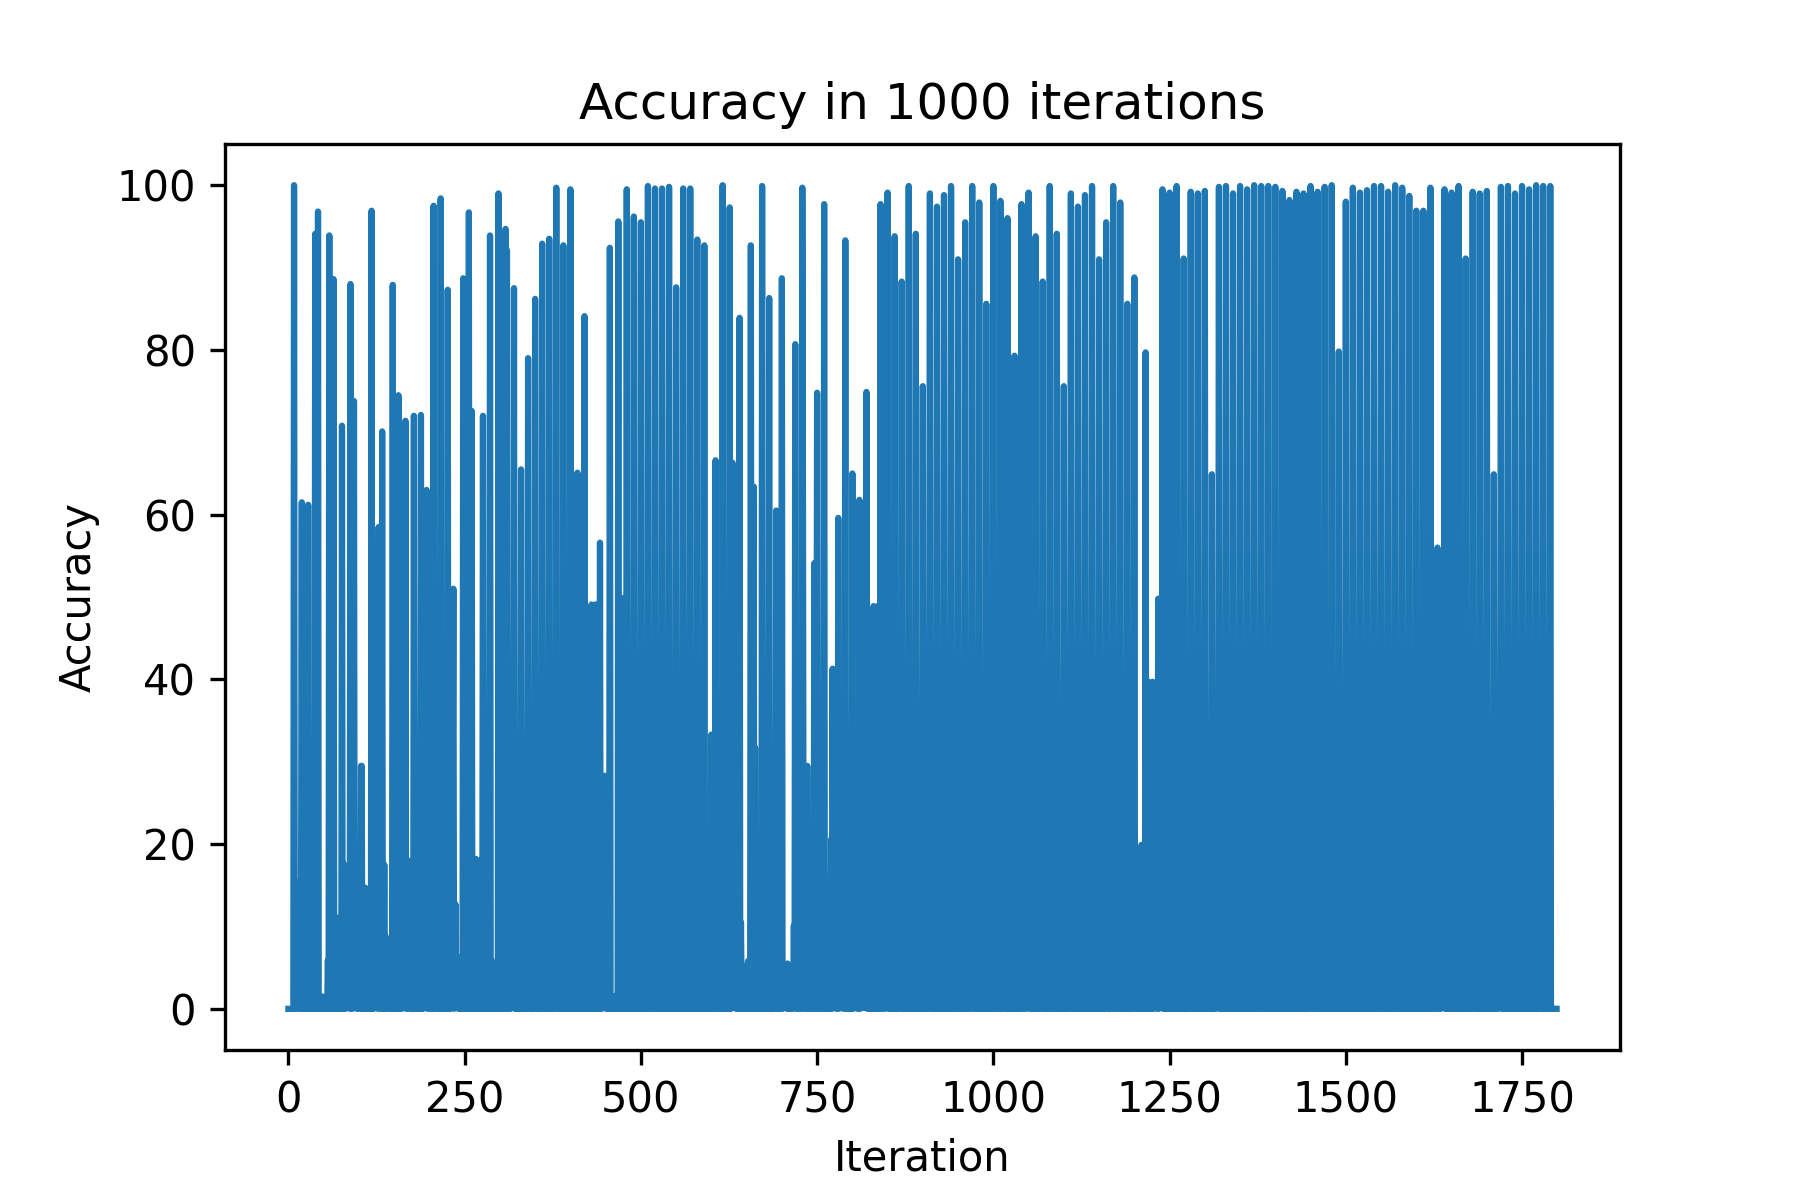
\includegraphics[width=\textwidth]{Images/plot_accuracy_1000.png}
         \caption{Plot of accuracy over 1000 iterations.}
         \label{fig:accuracy_1000}
     \end{subfigure}
     \hfill
        \caption{Plot of the percentage of accuracy.}
        \label{plot_accuracy}
\end{figure}


\clearpage
\newpage
\mbox{~}
\clearpage
\newpage

      \chapter{Conclusion}
\label{cha:conclusion}

\quad This thesis introduces the idea of continuous learning on micro-controllers for self-learning ML models. Device deployment in settings with variable context is frequent in TinyML apps. The change of context can cause the models' accuracy to deteriorate rapidly, making for unsuitable and unreliable gadgets. It is vital to use ongoing learning techniques in these situations. These support the models by giving the system flexibility and adaptability traits that can keep up with context drift. 
This study implements a CL strategy, particularly the TinyOL method. The algorithm is developed in a framework and deployed on the Max78000 micro-controller. The MCU uses a CNN accelerator to compute the inferences of new samples, paired with the CL system developed. 
In the application, the CL is applied for image classifications. Initially, the application uses other frameworks (such as PyTorch) to train the model to recognize digits. Later the CL system is used to recognize and replace a new class, the letter A from the Emnist dataset. 
The application is implemented in a supervised environment. The sample data are known to the user, and thanks to this knowledge, it was possible to deploy a pre-made true-label table. After a few training sessions, the method showed that the model accounted properly for each class. 
 
 \singlespacing
 
\quad One of the main drawbacks of this study is the loss of time between the loading and unloading of data. The time lost is due to the complex memory map of the CNN accelerator. To overcome the time problem there would be needed a deep memory scan, thanks to which it would be possible to update the weights and biases directly in the memory. A possible future implementation is the development of a streaming mode from a real-time camera. The problem with a camera would be the unsupervised environment in which a truth table can't be used. For this reason, the application in real-time settings has not yet been developed. 
 
\clearpage
\newpage
\mbox{~}
\clearpage
\newpage
      
    \endgroup


    % bibliografia in formato bibtex
    %
    % aggiunta del capitolo nell'indice
    \addcontentsline{toc}{chapter}{Bibliography}
    % stile con ordinamento alfabetico in funzione degli autori
    % \cite{Max78000}
    % \cite{MaximIntegratedAI}
    % \cite{deng2012mnist}
    % \cite{cohen2017emnist}
    % \cite{Quantum_machine_learning}
    % \cite{Continual_Learning_on_Max78000_Microcontroller}
    \bibliography{biblio}
    \bibliographystyle{plain}
%%%%%%%%%%%%%%%%%%%%%%%%%%%%%%%%%%%%%%%%%%%%%%%%%%%%%%%%%%%%%%%%%%%%%%%%%%
%%%%%%%%%%%%%%%%%%%%%%%%%%%%%%%%%%%%%%%%%%%%%%%%%%%%%%%%%%%%%%%%%%%%%%%%%%
%% Nota
%%%%%%%%%%%%%%%%%%%%%%%%%%%%%%%%%%%%%%%%%%%%%%%%%%%%%%%%%%%%%%%%%%%%%%%%%%
%% Nella bibliografia devono essere riportati tutte le fonti consultate 
%% per lo svolgimento della tesi. La bibliografia deve essere redatta 
%% in ordine alfabetico sul cognome del primo autore. 
%% 
%% La forma della citazione bibliografica va inserita secondo la fonte utilizzata:
%% 
%% LIBRI
%% Cognome e iniziale del nome autore/autori, la data di edizione, titolo, casa editrice, eventuale numero dell’edizione. 
%% 
%% ARTICOLI DI RIVISTA
%% Cognome e iniziale del nome autore/autori, titolo articolo, titolo rivista, volume, numero, numero di pagine.
%% 
%% ARTICOLI DI CONFERENZA
%% Cognome e iniziale del nome autore/autori (anno), titolo articolo, titolo conferenza, luogo della conferenza (città e paese), date della conferenza, numero di pagine. 
%% 
%% SITOGRAFIA
%% La sitografia contiene un elenco di indirizzi Web consultati e disposti in ordine alfabetico. 
%% E’ necessario:
%%   Copiare la URL (l’indirizzo web) specifica della pagina consultata
%%   Se disponibile, indicare il cognome e nome dell’autore, il titolo ed eventuale sottotitolo del testo
%%   Se disponibile, inserire la data di ultima consultazione della risorsa (gg/mm/aaaa).    
%%%%%%%%%%%%%%%%%%%%%%%%%%%%%%%%%%%%%%%%%%%%%%%%%%%%%%%%%%%%%%%%%%%%%%%%%%
%%%%%%%%%%%%%%%%%%%%%%%%%%%%%%%%%%%%%%%%%%%%%%%%%%%%%%%%%%%%%%%%%%%%%%%%%%
    

    \titleformat{\chapter}
        {\normalfont\Huge\bfseries}{Allegato \thechapter}{1em}{}
    % sezione Allegati - opzionale
    \appendix

\end{document}
